\documentclass[12pt,a4paper]{article}

% ── Packages ──────────────────────────────────────────────────────────────
\usepackage[margin=2.5cm]{geometry}
\usepackage{amsmath,amssymb,amsfonts}
\usepackage{graphicx}
\usepackage{booktabs}
\usepackage{siunitx}
\usepackage{xcolor}
\usepackage{caption}
\usepackage{subcaption}
\usepackage{setspace}

%\usepackage{lineno}
\usepackage[numbers,sort&compress]{natbib}
\usepackage[colorlinks=true,
            linkcolor=blue!60!black,
            citecolor=blue!60!black,
            urlcolor=blue!60!black]{hyperref}
\usepackage{array}
\usepackage{tabularx}
\usepackage{multirow}

% ── Typography ────────────────────────────────────────────────────────────
\onehalfspacing
\setlength{\parindent}{1.5em}
\setlength{\parskip}{2pt}

% ── Maths shortcuts ───────────────────────────────────────────────────────
\newcommand{\Tg}{T_{\mathrm{g}}}
\newcommand{\Tbat}{T_{\mathrm{cyc}}}
\newcommand{\rbar}{\bar{r}}
\newcommand{\sigr}{\sigma_r}
\newcommand{\rmax}{r_{\max}}
\newcommand{\rmin}{r_{\min}}
\newcommand{\Rsq}{R^2}
\newcommand{\degpp}{\,\text{pp}}
\newcommand{\siounit}[1]{\si{#1}}
\newcommand{\xcontam}{\chi}
\newcommand{\LJ}{Lennard-Jones}
\newcommand{\vtau}{\tau_{\mathrm{mem}}}
\newcommand{\Tzero}{T_0}  
\newcommand{\doi}[1]{\href{https://doi.org/#1}{doi:#1}}

% ── Colours ───────────────────────────────────────────────────────────────
\definecolor{darkblue}{RGB}{31,78,121}
\definecolor{darkred}{RGB}{192,57,43}
\definecolor{darkgreen}{RGB}{39,174,96}

% ─────────────────────────────────────────────────────────────────────────
\begin{document}

%\linenumbers

% ══════════════════════════════════════════════════════════════════════════
%  TITLE PAGE
% ══════════════════════════════════════════════════════════════════════════
\begin{titlepage}
\centering
\vspace*{1.5cm}

{\LARGE\bfseries Geometric Orthogonality of Competing Structural\\[6pt]
Memories in Glass: Temperature Controls\\[6pt]
Mechanical Erasure of Thermal History\par}

\vspace{1.4cm}

{\large Saurab Singh\textsuperscript{1}}

\vspace{0.6cm}

{\normalsize
\textsuperscript{1}Independent Researcher\\
\href{mailto:saurabsingh778@gmail.com}{saurabsingh778@gmail.com}
}

\vspace{1.2cm}

{\small \today}

\vspace{2.5cm}

\begin{abstract}
\noindent
Glass retains memory of its entire processing history in the spatial arrangement of atomic bonds.
Whether competing histories --- thermal (cooling rate) and mechanical (cyclic fatigue) --- encode in geometrically independent structural subspaces, or whether one erases the other, has not been systematically investigated.
Here we address this question using \LJ\ model glasses subjected to a 2D parameter sweep: strain amplitude $\delta \in \{4, 6, 8, 12\}\%$ and cycling temperature $\Tbat \in \{0.35, 0.38, 0.40, 0.42, 0.44, 0.46\}$ (in LJ reduced units, spanning $0.78$--$1.02\,\Tg$).
A GATv2 graph neural network trained on 8-dimensional local bond-length statistics simultaneously recovers both thermal and mechanical histories from a single atomic-configuration snapshot, losing less than $3$ percentage points of accuracy on either task relative to single-task baselines, and exhibiting cross-contamination below $0.21$ in all nine experimental conditions.
Latent-space principal component analysis confirms that the two histories occupy distinct latent directions in every condition studied.
Despite this geometric orthogonality, the detectability of thermal history is progressively degraded by cyclic fatigue: the cooling-rate classification accuracy on maximally fatigued glasses drops $14$--$31$ percentage points compared to pristine glasses.
Critically, this interference is controlled by the cycling temperature rather than the strain amplitude: temperature varied from $0.78\,\Tg$ to $1.02\,\Tg$ drives the drop from $14\degpp$ to $31\degpp$, while strain amplitude varied from $4\%$ to $12\%$ produces no systematic effect.
Confusion-matrix asymmetry analysis reveals a sharp mechanistic crossover at $\Tg$: below $\Tg$, cyclic strain preferentially drives fast-cooled glasses toward the slow-cooled structural attractor (palimpsest / mechanical annealing, $\alpha = +0.24$ to $+0.46$), while above $\Tg$ both histories are erased symmetrically by thermal re-equilibration ($\alpha = -0.05$, consistent with zero).
At the lowest temperature ($T = 0.35$, $0.78\,\Tg$), thermal history measurably modulates the learnability of the fatigue trajectory, consistent with the same mechanical-annealing mechanism.
Forgetting-curve analysis of the GNN accuracy as a function of fatigue-cycle number reveals that the thermal memory decay timescale $\vtau$ collapses super-Arrhenius-ally from $\vtau = 79$ cycles at $0.78\,\Tg$ to $\vtau = 11$ cycles at $0.89\,\Tg$; a Vogel-Tammann-Fulcher fit to the three sub-$\Tg$ timescales yields an ideal-glass temperature $\Tzero = 0.33$ (LJ units) and $R^2 = 0.999$, connecting the GNN structural probe quantitatively to the cooperative rearrangement dynamics of fragile glass.
These results establish that glass stores competing processing histories in geometrically orthogonal but not informationally independent subspaces, with the degree and \emph{direction} of cross-history interference governed by a thermally activated mechanism that undergoes a qualitative transition at $\Tg$, and whose kinetics are quantitatively described by the VTF law of fragile glass relaxation.
\end{abstract}

\vspace{1cm}

\noindent\textbf{Keywords:} glass structure, thermal history, cyclic fatigue, graph neural networks, structural memory, amorphous solids, potential energy landscape

\end{titlepage}

% ══════════════════════════════════════════════════════════════════════════
%  1.  INTRODUCTION
% ══════════════════════════════════════════════════════════════════════════
\section{Introduction}
\label{sec:intro}

Glasses are disordered solids whose properties depend sensitively on the path by which they were formed.
A glass produced by rapid quenching differs in mechanical stiffness, optical index, and ionic conductivity from one produced by slow annealing, even when their chemical compositions are identical~\cite{Debenedetti2001,Angell1995,Berthier2011}.
This \textit{thermal history dependence} has been studied for decades through the concept of fictive temperature~\cite{Tool1946,Narayanaswamy1971}: the effective temperature at which the supercooled liquid structure was frozen during cooling.
More recently, machine-learning probes have demonstrated that the fictive temperature is geometrically encoded in the distribution of local bond lengths and their spatial correlations, and is recoverable from a single configuration snapshot with high accuracy~\cite{Singh2025Paper1}.

In technological applications, however, glasses are rarely exposed to a single processing step.
Solid-state battery electrolytes — including lithium phosphorus oxynitride (LiPON), lithium garnet (LLZO), and related glass-ceramic materials — are manufactured by a thermal process and then subjected to thousands of electrochemical charge/discharge cycles, each of which drives volumetric strains of $3$--$8\%$ in the glass matrix~\cite{Janek2016,Yu2017,Sakamoto2013}.
The resulting \textit{cyclic mechanical fatigue} accumulates as irreversible atomic rearrangements that degrade ionic conductivity, promote dendrite formation, and ultimately cause battery failure~\cite{Porz2017,Zhao2020,Swamy2018}.
A companion study~\cite{Singh2025Paper2} demonstrated that this fatigue also leaves a geometric fingerprint detectable by the same GATv2 graph neural network (GNN) architecture used for thermal history, achieving $91$--$98\%$ classification accuracy between pristine and heavily fatigued glasses.

These two results together raise a fundamental question that neither study addresses: when both thermal and mechanical histories are present simultaneously, do they encode in the same geometric degrees of freedom (shared subspace, strong interference), or in structurally independent subspaces (geometric orthogonality)?
This question has direct practical implications: if the two histories compete for the same structural space, processing history is effectively overwritten by cycling; if they are orthogonal, a single snapshot in principle contains recoverable information about both.

The question is also theoretically significant.
The potential energy landscape (PEL) framework~\cite{Stillinger1995,Wales2003} distinguishes between the depth of an energy basin (set by thermal history) and its local geometry — the curvature and shape of the surrounding PEL (set by both thermal and mechanical history).
Thermal history primarily controls which basin the glass occupies; mechanical fatigue accumulates damage within and around that basin without necessarily relocating the system to a fundamentally different basin.
This physical picture suggests partial separation of the two histories in structure space, but the extent and parameter dependence of this separation have not been quantified.

Here we address this gap through a systematic computational study.
We generate \LJ\ model glasses with controlled thermal histories (fast vs.\ slow cooling, 100-fold difference in cooling time) and subject each to a cyclic volumetric strain protocol mimicking battery charge/discharge.
We then train GATv2 GNNs on 8-dimensional local bond-length statistics to simultaneously recover both histories from single snapshots, and characterise the latent space geometry using principal component analysis (PCA) and Spearman correlation.
Crucially, we vary two independent physical parameters — the cycling temperature $\Tbat$ and the strain amplitude $\delta$ — across nine experimental conditions, enabling a controlled measurement of what governs interference between the two histories.

Our principal findings are:
(i) the two histories consistently occupy distinct latent directions in all nine conditions, confirming geometric orthogonality;
(ii) the detectability of thermal history after fatigue is controlled by temperature rather than strain;
(iii) confusion-matrix asymmetry analysis reveals a sharp mechanistic crossover at $\Tg$ — below $\Tg$ fatigue acts as a directed annealing process (palimpsest), while above $\Tg$ both histories are erased symmetrically by thermal re-equilibration (amnesia);
and (iv) at the lowest temperatures, thermal history modulates the learnability of the fatigue trajectory, a subtle cross-history interaction consistent with the same mechanical-annealing mechanism;
and (v) the thermal memory decay timescale $\vtau$, extracted from stretched-exponential fits to GNN accuracy forgetting curves, exhibits super-Arrhenius temperature dependence quantitatively described by a Vogel-Tammann-Fulcher (VTF) law with fitted ideal-glass temperature $\Tzero = 0.33$, establishing that the GNN structural probe tracks the cooperative rearrangement dynamics of fragile glass.
% ══════════════════════════════════════════════════════════════════════════
%  2.  METHODS
% ══════════════════════════════════════════════════════════════════════════
\section{Methods}
\label{sec:methods}

\subsection{Model System}
\label{sec:model}

All simulations use the single-component \LJ\ potential in reduced units ($\sigma = \epsilon = m = 1$):
\begin{equation}
U(r) = 4\epsilon \left[\left(\frac{\sigma}{r}\right)^{12} - \left(\frac{\sigma}{r}\right)^{6}\right], \quad r < r_c = 2.5\sigma.
\label{eq:LJ}
\end{equation}
The system consists of $N = 256$ particles in a cubic periodic box of side $L = (N/\rho)^{1/3} \approx 5.975\sigma$ at number density $\rho = 1.2\sigma^{-3}$.
At this density the glass transition temperature is $\Tg \approx 0.45$ in LJ reduced units~\cite{Kob1995}.
Dynamics are evolved using Brownian (overdamped Langevin) dynamics with timestep $\Delta t = 5 \times 10^{-4}$ and force clipping at $\pm 50\epsilon/\sigma$ for numerical stability.
Simulations are implemented in JAX~\cite{Bradbury2018} with JIT-compiled force kernels.

\subsection{Glass Generation}
\label{sec:glass-gen}

Pristine glasses are generated via linear cooling from $T_{\rm high} = 2.0$ (liquid state) to $T_{\rm low} = 0.10$ (deep glass state).
Two cooling rates are used:
\begin{itemize}
  \item \textbf{Fast-cooled glass:} 4{,}000 Brownian steps over the cooling interval ($\Gamma_{\rm fast} = 1.0$ in LJ units), followed by 2{,}000 equilibration steps at $T_{\rm low}$.
  \item \textbf{Slow-cooled glass:} 400{,}000 Brownian steps ($\Gamma_{\rm slow} = 0.01$), followed by 20{,}000 equilibration steps. The cooling-time ratio is $100\times$.
\end{itemize}
Particles are initialised on a slightly perturbed simple-cubic lattice to avoid hard-core overlaps.
We generate $N_g = 100$ independent realisations of each type.
All generated configurations are validated against ten physical checks: absence of NaN/Inf positions, periodic-box containment, hard-core clearance ($r > 0.75\sigma$), coordination number range $[6, 18]$, no isolated atoms, mean bond length $[0.95, 1.40]\sigma$, bond-length standard deviation $[0.05, 0.35]\sigma$, LJ energy per particle $[-10, -2]\epsilon$, non-crystallinity ($\sigr > 0.05\sigma$), and structural heterogeneity.
All 600 configurations (100 fast $\times$ 3 snapshots + 100 slow $\times$ 3 snapshots) pass all checks with $100\%$ acceptance rate.

\subsection{Cyclic Fatigue Protocol}
\label{sec:fatigue}

Each pristine glass is subjected to up to $N_{\rm cyc} = 400$ simulated charge/discharge cycles.
One cycle consists of two phases:
\begin{enumerate}
  \item \textbf{Charge (expansion):} Atomic coordinates and box dimensions are affinely scaled by $(1 + \delta)$. Brownian dynamics are run for $N_{\rm step} = 500$ steps at temperature $\Tbat$.
  \item \textbf{Discharge (compression):} Coordinates are affinely compressed to the original box size. Dynamics continue for $N_{\rm step}$ steps at $\Tbat$.
\end{enumerate}
Affine scaling is the standard mechanical-deformation technique in molecular dynamics simulations of glasses~\cite{Lemaitre2006,Maloney2006}.
Snapshots are saved at cycles $c \in \{0, 200, 400\}$, yielding 600 graphs per experimental condition (100 fast + 100 slow glasses, 3 snapshots each).

The cycling temperature $\Tbat$ is varied across six values spanning the sub-$\Tg$ and near-$\Tg$ regimes:
\begin{equation}
\Tbat \in \{0.35,\; 0.38,\; 0.40,\; 0.42,\; 0.44,\; 0.46\} \quad (\text{in LJ reduced units}),
\end{equation}
corresponding to $T/\Tg \in \{0.78, 0.84, 0.89, 0.93, 0.98, 1.02\}$.
The strain amplitude is varied independently across four values:
\begin{equation}
\delta \in \{0.04,\; 0.06,\; 0.08,\; 0.12\},
\end{equation}
with $\delta = 0.08$ (8\%) and $\Tbat = 0.42$ serving as the reference (``baseline'') condition shared by both sweeps.
This yields nine distinct experimental conditions in total.

\textbf{Structural validation across cycles.}
We verify that fatigue accumulates physically by confirming that the bond-length standard deviation $\sigr$ is non-decreasing from cycle 0 to cycle 400 in the ensemble average, subject to a tolerance of $0.025\sigma$ to accommodate the ``conditioning dip'' documented in real battery electrolytes~\cite{Sakamoto2013}: fast-cooled glasses, starting in high-disorder configurations, may partially relax during early cycles before fatigue dominates.
This dip occurs in 21--30\% of fast-cooled glasses across conditions and is a known physical phenomenon, not a simulation artifact.

\subsection{Feature Extraction}
\label{sec:features}

For each configuration snapshot, we compute 8-dimensional local bond-length statistics per atom.
Let $\mathcal{N}(i)$ denote the first-shell neighbours of atom $i$ within cutoff $r_c = 1.5\sigma$ (corresponding to the first coordination shell at $\rho = 1.2$), and let $\{r_{ij}\}_{j \in \mathcal{N}(i)}$ be the set of bond lengths.
The node feature vector for atom $i$ is:
\begin{equation}
\mathbf{x}_i = \left[\bar{r}_i,\; \sigma_{r,i},\; r_{i}^{\min},\; r_{i}^{\max},\; \tilde{d}_i,\; \tilde{\gamma}_{1,i},\; Q_{25,i},\; Q_{75,i}\right]^\top \in \mathbb{R}^8,
\label{eq:features}
\end{equation}
where $\bar{r}_i = \langle r_{ij} \rangle$ is the mean bond length, $\sigma_{r,i}$ its standard deviation, $r_i^{\min}$ and $r_i^{\max}$ are extremal bond lengths, $\tilde{d}_i = d_i / d_{\max}$ is the normalised coordination number, $\tilde{\gamma}_{1,i} = \text{clip}(\mu_3^i / (\sigma_{r,i}^3 + \epsilon), -5, 5)$ is a skewness proxy (with $\mu_3^i$ the third central moment), and $Q_{25,i}$, $Q_{75,i}$ are the 25th and 75th percentiles of the bond-length distribution.

\textbf{Instance normalisation.}
All features are normalised per graph using z-score standardisation:
\begin{equation}
\mathbf{x}_i \leftarrow \frac{\mathbf{x}_i - \boldsymbol{\mu}^{(s)}}{\boldsymbol{\sigma}^{(s)} + \epsilon},
\label{eq:instnorm}
\end{equation}
where $\boldsymbol{\mu}^{(s)}$ and $\boldsymbol{\sigma}^{(s)}$ are the mean and standard deviation of the feature vectors across all atoms in graph $s$.
This operation removes all global magnitude information — absolute bond-length scales, global density — forcing the model to rely exclusively on the \emph{relational geometry} of the local bond network.
As demonstrated in the companion studies~\cite{Singh2025Paper1,Singh2025Paper2}, instance normalisation consistently improves classification accuracy and stabilises training.
Edge attributes $e_{ij} = r_{ij}$ (raw bond lengths, not normalised) are passed directly to the GNN.

\subsection{Graph Neural Network Architecture}
\label{sec:gnn}

We employ GATv2~\cite{Brody2021} as the message-passing backbone.
A shared encoder maps node features to a 64-dimensional embedding:
\begin{equation}
\mathbf{h}_i^{(0)} = \mathbf{W}_{\rm enc}\,\mathbf{x}_i,
\end{equation}
followed by two GATv2 layers with 4 attention heads each and edge dimension 1:
\begin{align}
\mathbf{h}_i^{(1)} &= \mathrm{GATv2}^{(1)}\!\left(\{\mathbf{h}_j^{(0)}, e_{ij}\}_{j \in \mathcal{N}(i)}\right) \in \mathbb{R}^{256}, \\
\mathbf{h}_i^{(2)} &= \mathrm{GATv2}^{(2)}\!\left(\{\mathbf{h}_j^{(1)}, e_{ij}\}_{j \in \mathcal{N}(i)}\right) \in \mathbb{R}^{256}.
\end{align}
Graph-level representations are obtained by global mean pooling:
\begin{equation}
\mathbf{h}_{\rm graph} = \frac{1}{N} \sum_{i=1}^N \mathbf{h}_i^{(2)},
\end{equation}
followed by a post-message-passing MLP:
\begin{equation}
\mathbf{z} = \mathrm{ReLU}\!\left(\mathbf{W}_2 \,\mathrm{ReLU}\!\left(\mathrm{LN}\!\left(\mathbf{W}_1\,\mathbf{h}_{\rm graph}\right)\right)\right) \in \mathbb{R}^{64},
\label{eq:latent}
\end{equation}
with LayerNorm (LN) and Dropout($p=0.2$) in the first sub-layer.
The 64-dimensional vector $\mathbf{z}$ is the shared latent representation used for all analyses.

\textbf{Multi-task output heads.}
For the multi-task classifier (Experiments 2 and 3), two linear heads operate on $\mathbf{z}$:
\begin{align}
\hat{y}_{\rm cool} &= \mathbf{w}_{\rm cool}^\top \mathbf{z} \in \mathbb{R} \quad (\text{binary cooling: fast vs slow}), \\
\hat{\mathbf{y}}_{\rm fat} &= \mathbf{W}_{\rm fat}\,\mathbf{z} \in \mathbb{R}^3 \quad (\text{3-class fatigue: cycle 0, 200, 400}).
\end{align}
The training loss is:
\begin{equation}
\mathcal{L} = w_{\rm cool}\,\mathcal{L}_{\rm BCE}(\hat{y}_{\rm cool}, y_{\rm cool}) + w_{\rm fat}\,\mathcal{L}_{\rm CE}(\hat{\mathbf{y}}_{\rm fat}, y_{\rm fat}),
\label{eq:loss}
\end{equation}
with $w_{\rm cool} = w_{\rm fat} = 1.0$ (equal weighting; this is a deliberate neutral choice).

\subsection{Training Protocol}
\label{sec:training}

All experiments use 5-fold stratified cross-validation (stratified on the combined label $\ell = 3y_{\rm cool} + y_{\rm fat} \in \{0,\ldots,5\}$, ensuring each fold contains equal proportions of all six history combinations).
Training hyperparameters: Adam optimiser, learning rate $3 \times 10^{-4}$, weight decay $10^{-4}$, cosine annealing scheduler, mixed-precision AMP, batch size 32, early stopping on validation loss with patience 25 epochs, maximum 150 epochs.
The dataset per condition consists of 600 graphs (100 fast + 100 slow glasses, 3 cycle snapshots each).

\subsection{Experimental Design}
\label{sec:expdesign}

Six experiments are conducted for each of the nine physical conditions:

\begin{description}
  \item[Exp 1A/1B: Single-task baselines.] Separate GATv2 classifiers for cooling (binary) and fatigue (3-class), providing the performance ceiling when each history is decoded in isolation.
  \item[Exp 2: Multi-task classification.] Joint GATv2 with two output heads, measuring the cost of simultaneous decoding.
  \item[Exp 3: Latent space orthogonality.] PCA of the 64-dimensional latent vectors $\{\mathbf{z}\}$ extracted from the multi-task model. Spearman rank correlations $\rho(\mathrm{PC}_k, y_{\rm cool})$ and $\rho(\mathrm{PC}_k, y_{\rm fat})$ are computed for $k = 1, \ldots, 10$. Cross-contamination is defined as:
  \begin{equation}
  \xcontam = \frac{|\rho(\mathrm{PC}_{k^*_{\rm fat}}, y_{\rm cool})| + |\rho(\mathrm{PC}_{k^*_{\rm cool}}, y_{\rm fat})|}{2},
  \label{eq:xcontam}
  \end{equation}
  where $k^*_{\rm cool}$ and $k^*_{\rm fat}$ are the PCs most correlated with each label. Low $\xcontam$ indicates orthogonal encoding; $\xcontam < 0.15$ is classified as ``strong'' orthogonality and $\xcontam < 0.30$ as ``partial''.
  \item[Exp 4: History dominance test.] A separate cooling classifier is trained on (a) pristine glasses only (cycle 0) and (b) maximally fatigued glasses (cycle 400). The drop in accuracy from (a) to (b) quantifies the degree to which fatigue overwrites thermal memory.
  
  \item[Exp 7: Confusion-matrix directionality.]
  For each condition, the Exp~4B cooling classifier (trained on cycle-400 glasses) is re-evaluated with per-sample prediction recording.
  The confusion matrix is extracted for each of the five cross-validation folds.
  The \emph{asymmetry ratio}
  \begin{equation}
    \alpha = \frac{P(\text{fast}\to\text{slow}) - P(\text{slow}\to\text{fast})}
                  {P(\text{fast}\to\text{slow}) + P(\text{slow}\to\text{fast})}
    \label{eq:alpha}
  \end{equation}
  is computed on pooled predictions across folds, where $P(\text{fast}\to\text{slow})$ is the fraction of fast-cooled glasses misclassified as slow (false positive rate) and $P(\text{slow}\to\text{fast})$ is the fraction of slow-cooled glasses misclassified as fast (false negative rate).
  Values $\alpha > 0$ indicate that fatigue preferentially transforms the fast-cooled structural signature toward the slow-cooled attractor (\emph{palimpsest} / mechanical annealing);
  $\alpha \approx 0$ indicates symmetric misclassification with no preferred direction (\emph{amnesia}).
  Bootstrap 95\% confidence intervals for $\alpha$ are computed using $2\,000$ resamples of the pooled prediction set.
  The Spearman rank correlation between $\alpha$ and the Exp~4 interference drop is computed across all nine conditions to test whether the mechanism and the magnitude of interference co-vary.
  \item[Exp 8: Forgetting curve and super-Arrhenius analysis.]
  For three cycling temperatures in the sub-$\Tg$ palimpsest regime ($T \in \{0.35, 0.38, 0.40\}$), a GATv2 binary cooling classifier is trained and evaluated separately on glasses at each of a dense set of cycle snapshots.
  For $T = 0.35$ the snapshots are $c \in \{0, 50, 100, 150, 200, 250, 300, 350, 400\}$ (9 points); for $T = 0.38$ and $T = 0.40$ the snapshots are $c \in \{0, 5, 10, 15, 20, 30, 40, 50, 75, 100, 150, 200\}$ (12 points, dense early sampling to resolve fast timescales).
  All datasets use 100 fast-cooled and 100 slow-cooled glasses per cycle point, evaluated under 5-fold stratified cross-validation with the same hyperparameters as the main experiments.
  The resulting GNN accuracy curve $a(c, T)$ — the probability of correctly recovering thermal history after $c$ fatigue cycles — constitutes the \emph{forgetting curve}.
  Each forgetting curve is fitted to a stretched exponential (Kohlrausch-Williams-Watts, KWW):
  \begin{equation}
    a(c, T) = A_\infty(T) + \bigl[A_0(T) - A_\infty(T)\bigr]\,
              \exp\!\left[-\left(\frac{c}{\vtau(T)}\right)^{\!\beta(T)}\right],
    \label{eq:kww}
  \end{equation}
  where $A_0$ is the pristine-glass accuracy (cycle 0), $A_\infty$ is the long-time plateau accuracy, $\vtau$ is the memory decay timescale (in fatigue cycles), and $\beta \in (0, 2]$ is the KWW stretching exponent.
  Fits are performed using weighted nonlinear least squares with fold-standard-deviation weights; convergence is declared when the fitted $\vtau$ is not at a bound and $R^2 > 0.5$.
  The three converged timescales $\{\vtau(T)\}$ are then fitted to the Vogel-Tammann-Fulcher (VTF) equation~\cite{Vogel1921,Fulcher1925,Tammann1926}:
  \begin{equation}
    \vtau(T) = {\vtau}_{\infty} \exp\!\left(\frac{D\,\Tzero}{T - \Tzero}\right),
    \label{eq:vtf}
  \end{equation}
  where $\Tzero$ is the ideal-glass (Kauzmann) temperature at which $\vtau$ diverges, $D$ is the kinetic fragility parameter, and ${\vtau}_{\infty}$ is the high-temperature limit.
  Temperatures $T \geq 0.42$ ($\geq 0.93\,\Tg$) are excluded from this analysis: at these temperatures the forgetting timescale falls below the minimum cycle-sampling interval of 5 cycles and cannot be resolved from single-snapshot data alone.
  The VTF fit is performed on $\log\vtau$ vs $1/(T - \Tzero)$ using a grid search over $\Tzero \in [0.28, 0.40]$ with step $0.01$, selecting the value that maximises $R^2$.
  \item[Exp 5: Fatigue regression.] GATv2 regression to predict the normalised cycle number $c/400 \in [0,1]$, trained separately on fast-cooled, slow-cooled, and all glasses. A difference in $R^2$ between fast and slow glasses indicates that thermal history modulates the learnability of the fatigue trajectory.
  \item[Exp 6: Permutation importance.] Post-hoc zero-out analysis on single-task cooling and fatigue classifiers. Each of the 8 features is zeroed across all nodes; the resulting AUC drop quantifies its importance. Comparing rankings between tasks reveals whether the two histories use different geometric degrees of freedom.
\end{description}

% ══════════════════════════════════════════════════════════════════════════
%  3.  RESULTS
% ══════════════════════════════════════════════════════════════════════════
\section{Results}
\label{sec:results}

\subsection{Structural Validation: Fatigue Accumulates Geometrically}
\label{sec:structural}

Before GNN training, we verify that the cycling protocol creates physically meaningful structural changes.
Across all nine conditions, the bond-length standard deviation $\sigr$ increases monotonically from cycle 0 to cycle 400 in the ensemble average, with the net increase ranging from $0.0023\sigma$ (slow-cooled, $\delta=8\%$, $\Tbat=0.42$) to $0.0096\sigma$ (fast-cooled, $\delta=4\%$, $\Tbat=0.42$).
The mean bond length remains essentially constant (change $<0.1\%$), confirming that fatigue manifests as bond-length disorder rather than bulk volume change.
This is consistent with the companion study~\cite{Singh2025Paper2} and with experimental observations of conditioning in solid electrolytes~\cite{Sakamoto2013}.

Importantly, 21--30\% of fast-cooled glasses exhibit a ``conditioning dip'' — a transient decrease in $\sigr$ during the first 200 cycles — before net disorder accumulates.
This effect, absent or much weaker ($<0.003\sigma$) in slow-cooled glasses, reflects the fact that fast-cooled glasses start in far-from-equilibrium configurations: early cycles inject enough mechanical energy to allow partial relaxation before plastic damage accumulates.
The asymmetry between fast and slow glasses in early-cycle behaviour foreshadows the regression asymmetry found in Experiment 5 at low temperatures (Section~\ref{sec:regression}).

\subsection{Single-Task Baselines}
\label{sec:singletask}

Single-task GATv2 classifiers achieve the following accuracies on the baseline condition ($\delta = 8\%$, $\Tbat = 0.42$):
cooling, $80.3 \pm 4.96\%$ (AUC $= 0.890$); fatigue (3-class), $68.3 \pm 2.17\%$ (macro-F1 $= 0.665$).
Both are substantially above their respective chance levels (50\% and 33.3\%).
Across all nine conditions, single-task cooling accuracy ranges from 77.3\% (at $\Tbat = 0.46$, near/above $\Tg$) to 82.8\% ($\Tbat = 0.35$), and single-task fatigue accuracy from 64.5\% to 68.7\%.

The relatively modest cooling accuracy (compared to the $>95\%$ achieved in the companion thermal-history study~\cite{Singh2025Paper1}) reflects the deliberate design choice: the multi-history dataset contains 3 cycle snapshots per glass, not just the pristine state.
In the pristine (cycle 0) subset alone, cooling accuracy reaches 92--95\% (Exp 4A), consistent with the companion study.
The lower overall accuracy on the mixed dataset arises because fatigued glasses partially obscure the thermal signature, which is precisely the interference phenomenon this study aims to characterise.

\subsection{Multi-Task Decoding: Near-Lossless Simultaneous Recovery}
\label{sec:multitask}

\begin{table}[htbp]
\centering
\caption{Multi-task versus single-task accuracy across all nine conditions. ``Gap'' is single-task minus multi-task accuracy (pp). All values are 5-fold CV means. Negative gaps indicate multi-task outperforms single-task. All gaps are below $3\degpp$.}
\label{tab:multitask}
\begin{tabular}{lcccccc}
\toprule
Condition & ST Cool & MT Cool & Gap & ST Fat & MT Fat \\
          & (\%)    & (\%)    & (pp) & (\%)  & (\%) \\
\midrule
\multicolumn{6}{l}{\textit{Temperature sweep ($\delta = 8\%$)}} \\
$T = 0.35$ ($0.78\,\Tg$) & 82.8 & 81.7 & $+1.1$ & 64.5 & 65.8 \\
$T = 0.38$ ($0.84\,\Tg$) & 82.2 & 82.3 & $-0.1$ & 66.5 & 65.0 \\
$T = 0.40$ ($0.89\,\Tg$) & 81.2 & 80.7 & $+0.5$ & 66.0 & 66.2 \\
$T = 0.42$ ($0.93\,\Tg$, baseline) & 80.3 & 79.7 & $+0.7$ & 68.3 & 67.5 \\
$T = 0.44$ ($0.98\,\Tg$) & 81.8 & 81.7 & $+0.1$ & 64.8 & 66.3 \\
$T = 0.46$ ($1.02\,\Tg$) & 77.3 & 74.5 & $+2.8$ & 68.5 & 66.7 \\
\midrule
\multicolumn{6}{l}{\textit{Strain sweep ($\Tbat = 0.42$)}} \\
$\delta = 4\%$ & 81.5 & 81.8 & $-0.3$ & 68.7 & 66.8 \\
$\delta = 6\%$ & 79.8 & 80.7 & $-0.8$ & 64.7 & 61.0 \\
$\delta = 8\%$ (baseline) & 80.3 & 79.7 & $+0.7$ & 68.3 & 67.5 \\
$\delta = 12\%$ & 80.0 & 77.7 & $+2.3$ & 66.7 & 63.2 \\
\bottomrule
\end{tabular}
\end{table}

The multi-task GATv2 recovers both histories simultaneously with accuracy losses below $3\degpp$ in every condition (Table~\ref{tab:multitask}).
In seven of nine temperature-and-strain conditions the gap is below $1.5\degpp$; the largest gaps occur at $\Tbat = 0.46$ ($+2.8\degpp$) and $\delta = 12\%$ ($+2.3\degpp$), both still within fold-to-fold variance.
Notably, in four conditions the multi-task model \emph{outperforms} the single-task baseline on cooling (negative gaps), suggesting that fatigue supervision acts as a regulariser.
These results establish that simultaneous decoding of both histories from a single snapshot is achievable with negligible accuracy cost across the full parameter space studied.

\subsection{Latent Space Orthogonality}
\label{sec:orthogonality}

Figure~\ref{fig:fig3} summarises the cross-contamination metric $\xcontam$ (Eq.~\ref{eq:xcontam}) across all conditions.

\begin{figure}[htbp]
\centering
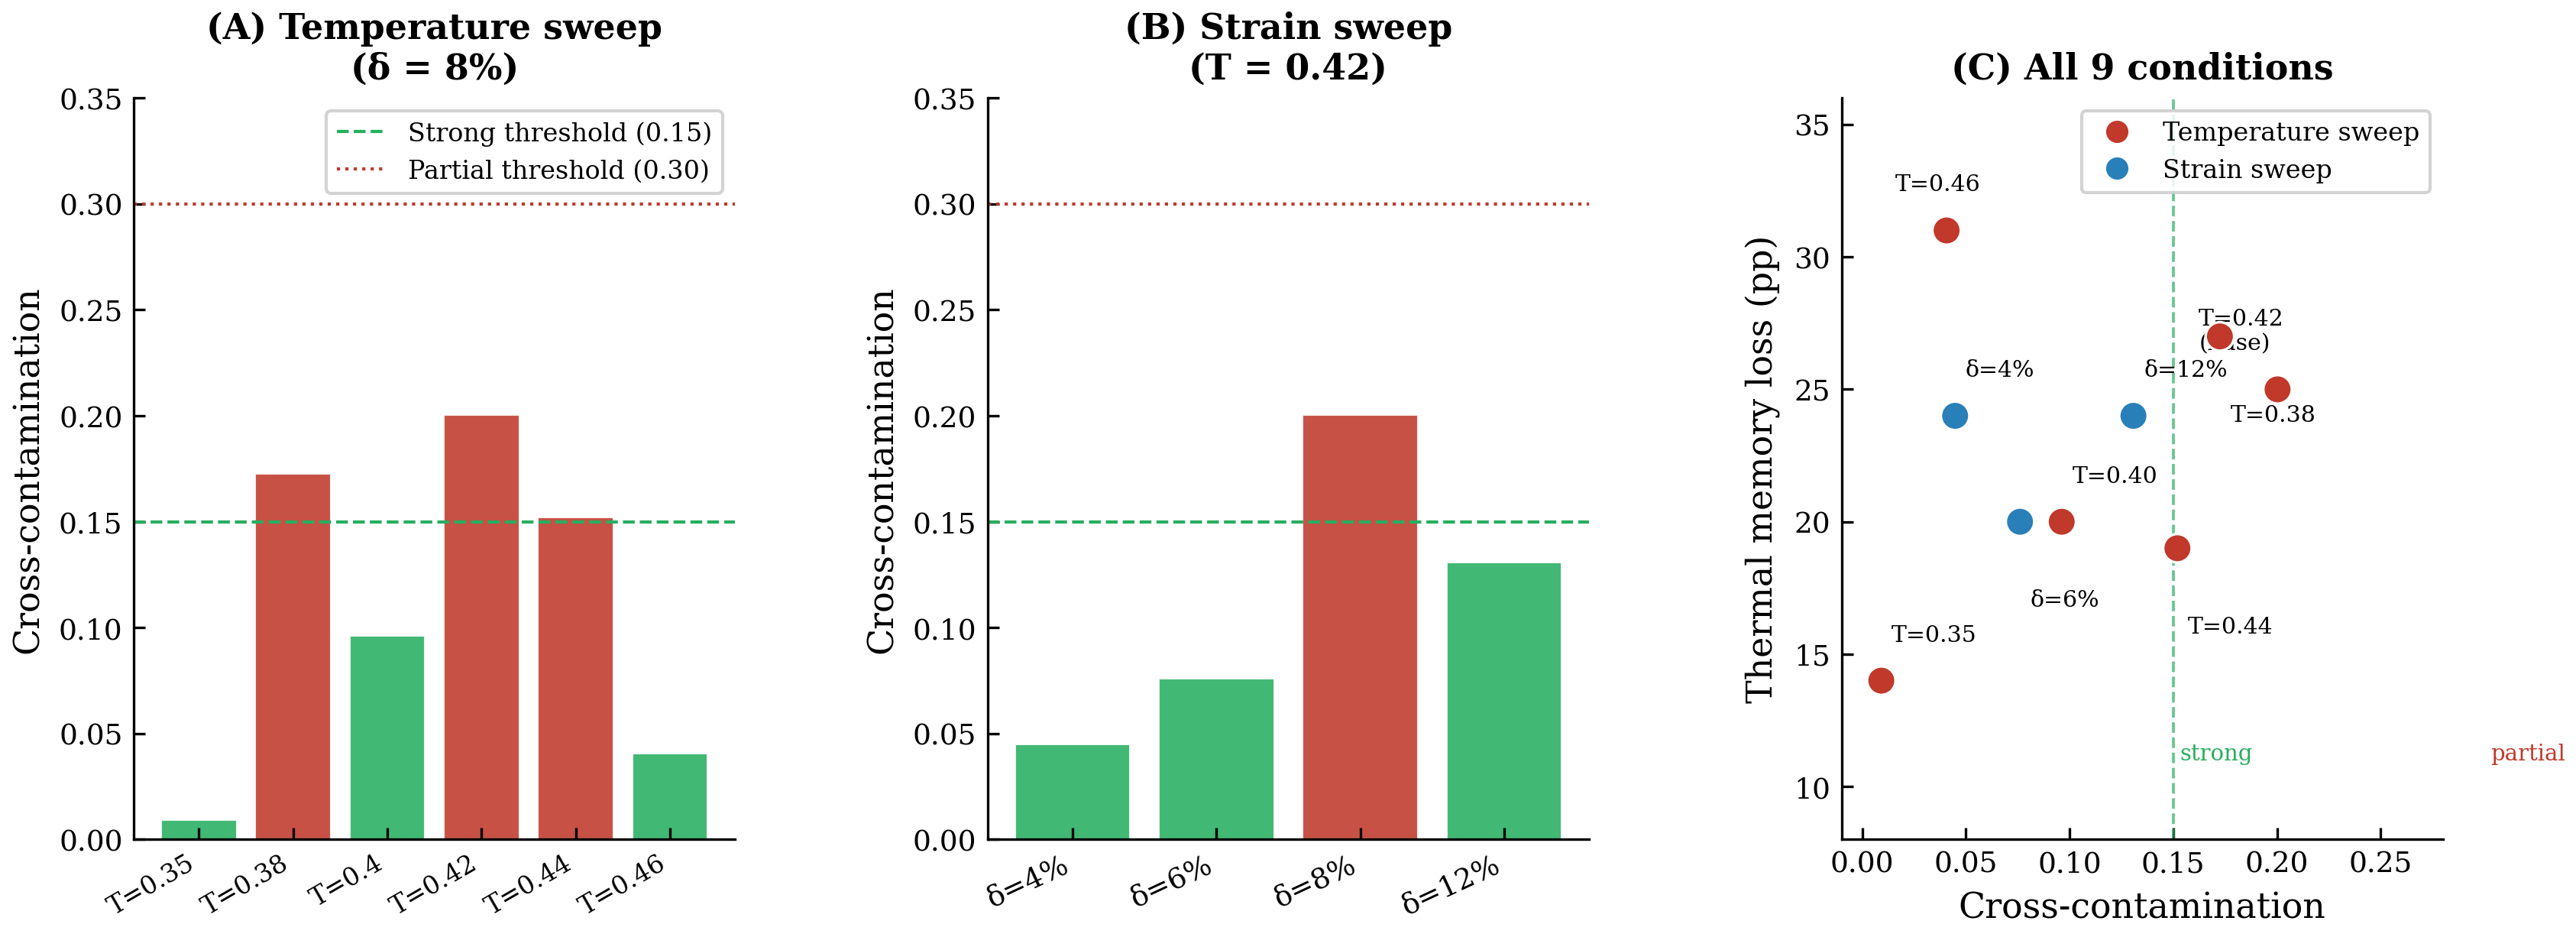
\includegraphics[width=\linewidth]{fig3_orthogonality.png}
\caption{Latent space orthogonality across all nine experimental conditions.
(A) Cross-contamination $\xcontam$ for the temperature sweep ($\delta = 8\%$), with six bars corresponding to $T \in \{0.35, 0.38, 0.40, 0.42, 0.44, 0.46\}$.
(B) Cross-contamination for the strain sweep ($\Tbat = 0.42$).
(C) Scatter of $\xcontam$ against interference drop (Exp 4) for all nine conditions.
Dashed and dotted lines mark the strong ($\xcontam < 0.15$) and partial ($\xcontam < 0.30$) orthogonality thresholds.
In all nine conditions, the histories occupy distinct principal components ($k^*_{\rm cool} \neq k^*_{\rm fat}$); $\xcontam$ never exceeds $0.21$.}
\label{fig:fig3}
\end{figure}

In all nine conditions, the best principal component for cooling ($k^*_{\rm cool}$) differs from the best for fatigue ($k^*_{\rm fat}$), and $\xcontam$ remains below $0.21$.
Six of nine conditions satisfy the strong orthogonality criterion ($\xcontam < 0.15$); the remaining three (baseline at $\Tbat = 0.42$, $\Tbat = 0.38$, and $\Tbat = 0.44$) satisfy partial orthogonality ($\xcontam < 0.30$).

Importantly, Panel C of Figure~\ref{fig:fig3} reveals that $\xcontam$ and the interference drop (Exp 4, Section~\ref{sec:dominance}) are not correlated across conditions.
For example, $\Tbat = 0.46$ produces the largest drop ($31\degpp$) yet has one of the lowest contaminations ($\xcontam = 0.041$); conversely, $\Tbat = 0.38$ produces both high drop ($27\degpp$) and relatively high contamination ($\xcontam = 0.173$).
This decorrelation indicates that latent-space orthogonality and feature-level interference are distinct phenomena: the GNN can organise its latent space to separate the two histories even when the underlying bond-length features are partially shared between tasks.

\subsection{History Dominance: Temperature Controls Interference}
\label{sec:dominance}

The core experimental result is shown in Figure~\ref{fig:fig1} and Table~\ref{tab:allresults}.

\begin{figure}[htbp]
\centering
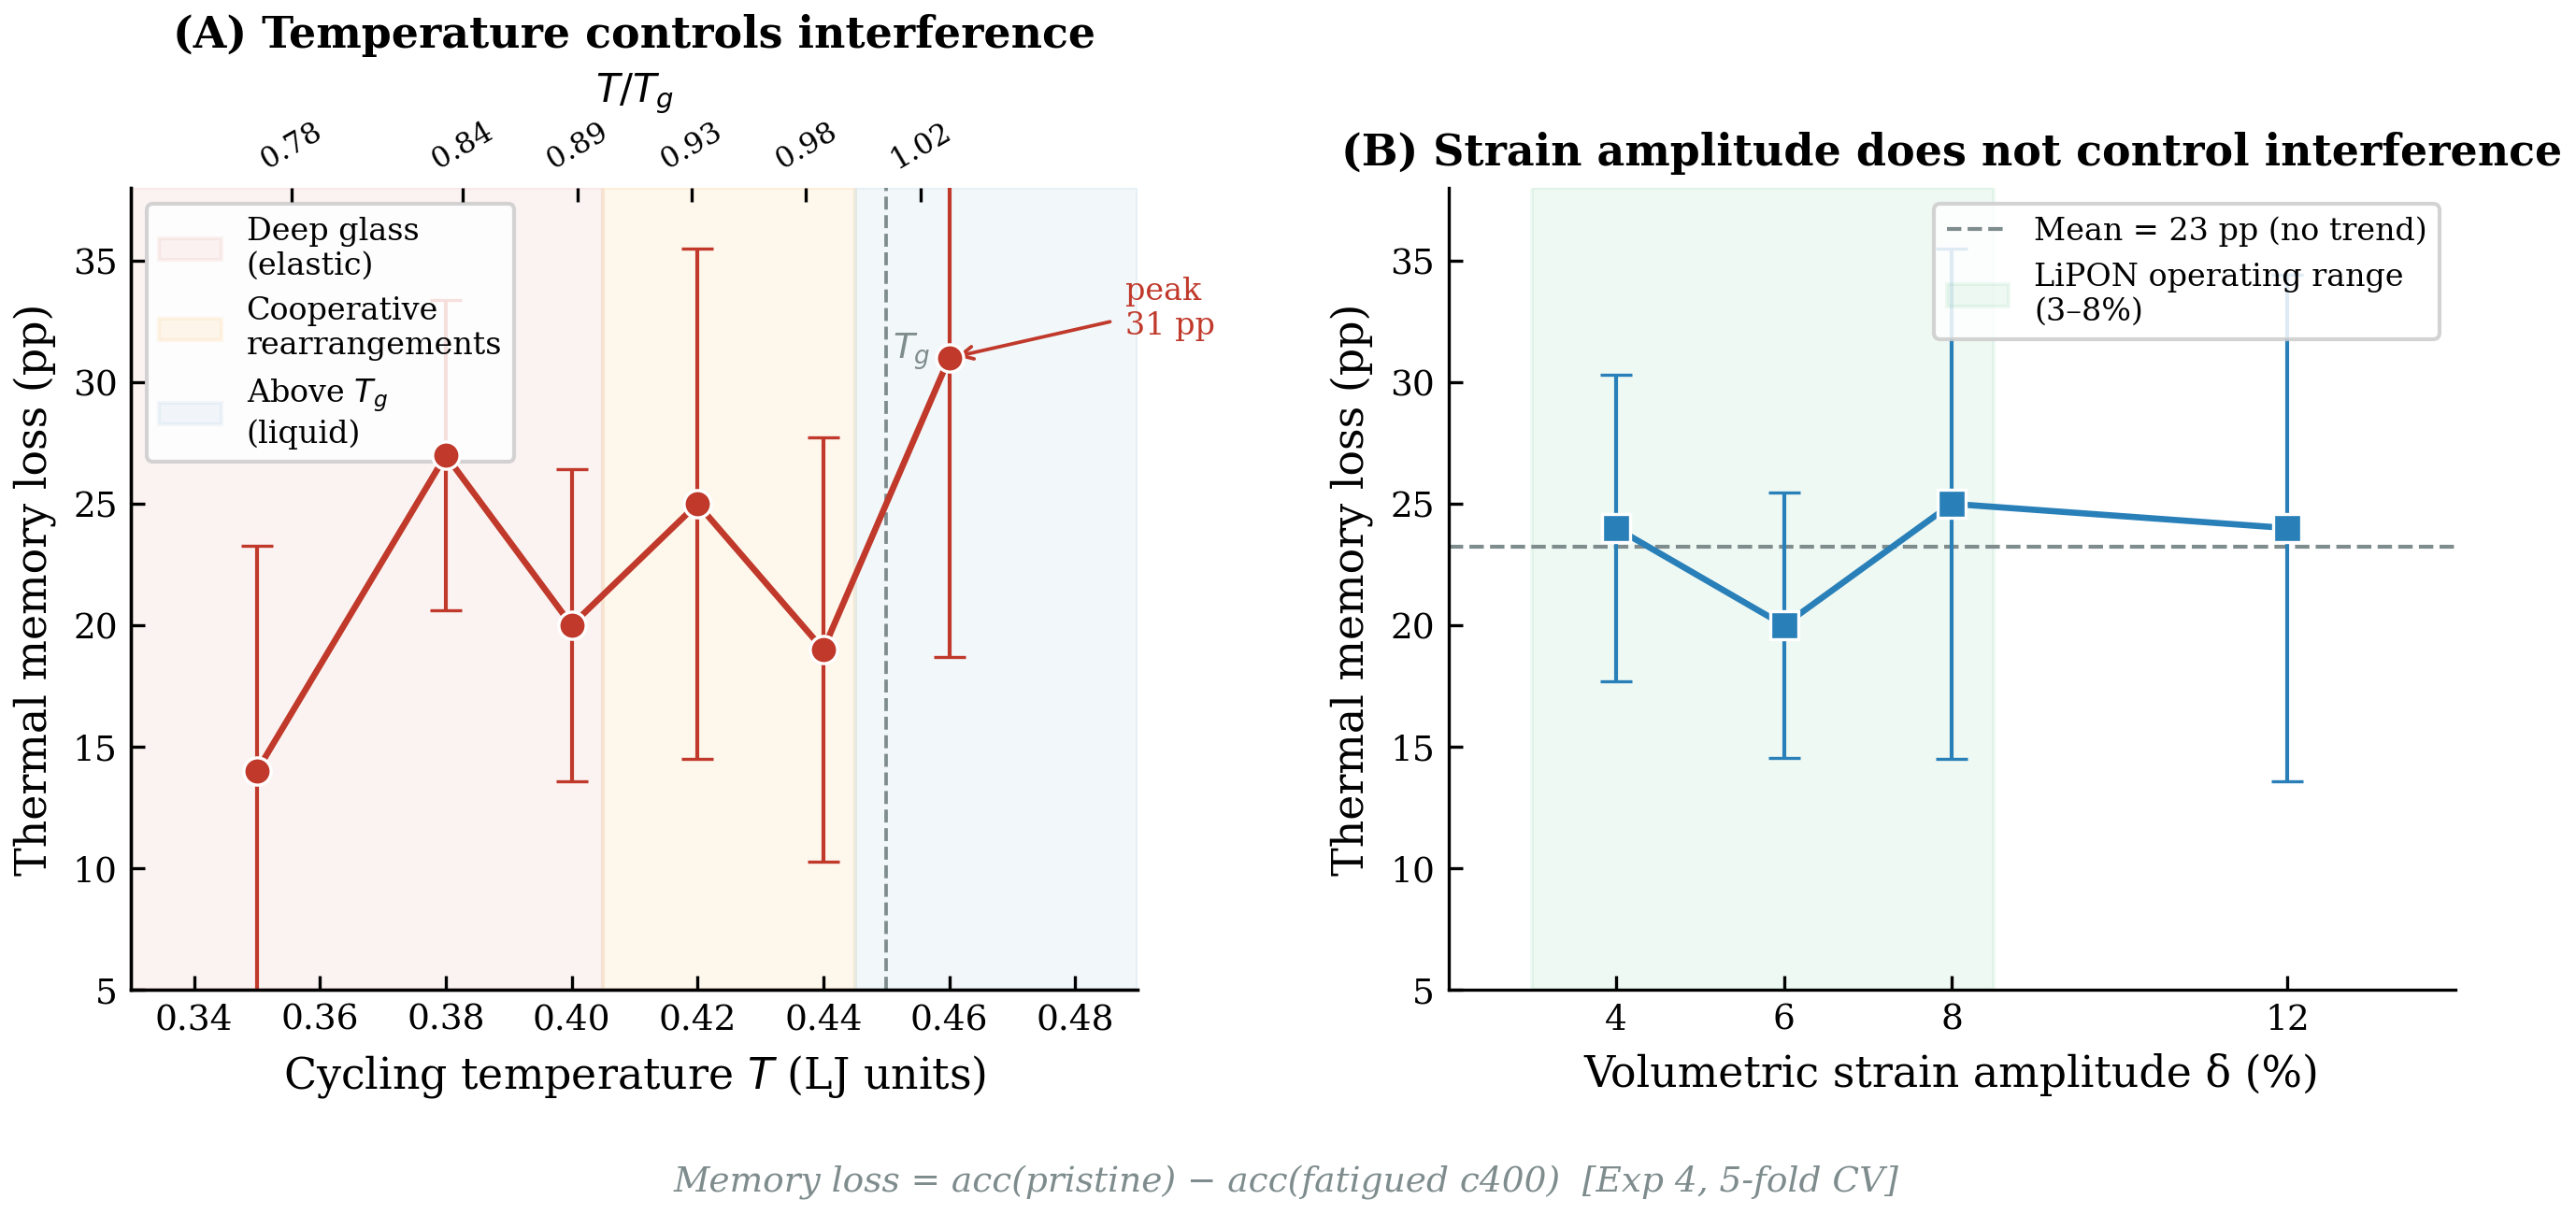
\includegraphics[width=\linewidth]{fig1_interference_map.png}
\caption{The interference map. Each point shows the drop in cooling-rate classification accuracy when the model is trained on maximally fatigued glasses (cycle 400) rather than pristine glasses (cycle 0).
(A) Temperature sweep ($\delta = 8\%$, six points): the drop increases broadly from $14\degpp$ at $T = 0.35$ ($0.78\,\Tg$) to $31\degpp$ at $T = 0.46$ ($1.02\,\Tg$), consistent with thermally activated erasure; condition-to-condition scatter (error bars: fold-SD) precludes identification of a sharp mechanistic crossover. Shaded regions mark the deep-glass, cooperative-rearrangement, and above-$\Tg$ regimes.
(B) Strain sweep ($\Tbat = 0.42$): the drop is statistically flat across $\delta = 4$--$12\%$, with a mean of $23\degpp$ and no discernible trend.}
\label{fig:fig1}
\end{figure}

\begin{table}[htbp]
\centering
\caption{Complete results across all nine experimental conditions. Acc$_{4A}$ = cooling accuracy on pristine glasses (cycle 0); Acc$_{4B}$ = cooling accuracy on maximally fatigued glasses (cycle 400); Drop = Acc$_{4A}$ $-$ Acc$_{4B}$ (percentage points); $\xcontam$ = cross-contamination (Eq.~\ref{eq:xcontam}); $R^2$ = fatigue regression $R^2$ on all glasses; Orth = orthogonality classification. All classification results are 5-fold CV means.}
\label{tab:allresults}
\begin{tabular}{lcccccc}
\toprule
Condition & Acc$_{4A}$ & Acc$_{4B}$ & Drop & $\xcontam$ & $R^2$ & Orth \\
          & (\%) & (\%) & (pp) & & & \\
\midrule
\multicolumn{7}{l}{\textit{Temperature sweep ($\delta = 8\%$)}} \\
$T = 0.35$ ($0.78\,\Tg$) & 92.0 & 78.0 & \textbf{14} & 0.009 & 0.673 & Strong \\
$T = 0.38$ ($0.84\,\Tg$) & 95.0 & 68.0 & 27 & 0.173 & 0.708 & Partial \\
$T = 0.40$ ($0.89\,\Tg$) & 93.5 & 73.5 & 20 & 0.096 & 0.720 & Strong \\
$T = 0.42$ ($0.93\,\Tg$) & 95.0 & 70.0 & 25 & 0.200 & 0.720 & Partial \\
$T = 0.44$ ($0.98\,\Tg$) & 93.5 & 74.5 & 19 & 0.152 & 0.729 & Partial \\
$T = 0.46$ ($1.02\,\Tg$) & 95.5 & 64.5 & \textbf{31} & 0.041 & 0.716 & Strong \\
\midrule
\multicolumn{7}{l}{\textit{Strain sweep ($\Tbat = 0.42$)}} \\
$\delta = 4\%$ & 94.0 & 70.0 & 24 & 0.045 & 0.726 & Strong \\
$\delta = 6\%$ & 92.5 & 72.5 & 20 & 0.076 & 0.714 & Strong \\
$\delta = 8\%$ (baseline) & 95.0 & 70.0 & 25 & 0.200 & 0.720 & Partial \\
$\delta = 12\%$ & 95.5 & 71.5 & 24 & 0.131 & 0.736 & Strong \\
\bottomrule
\end{tabular}
\end{table}

The most striking contrast is between Panels A and B of Figure~\ref{fig:fig1}: temperature drives a $17\degpp$ range of interference (from minimum $14\degpp$ at $T=0.35$ to maximum $31\degpp$ at $T=0.46$), while strain produces no systematic variation over a threefold range ($4$--$12\%$).

\textbf{Temperature dependence: a broad trend with condition-to-condition scatter.}
The interference drop values across the six temperature points are: $14$, $27$, $20$, $25$, $19$, $31\degpp$ (Table~\ref{tab:allresults}).
The overall direction is a broad increase from the lowest to the highest temperature, spanning a $17\degpp$ range and consistent with thermally activated structural erasure.
However, the intermediate points exhibit substantial scatter — the drop at $T = 0.40$ ($20\degpp$) is lower than at $T = 0.38$ ($27\degpp$), and the drop at $T = 0.44$ ($19\degpp$) is lower than at $T = 0.42$ ($25\degpp$) — which may reflect genuine condition-to-condition variability in irreversible rearrangement rates rather than a structured non-monotonic phenomenon.
The fold-to-fold standard deviations range from $\pm 6.4\degpp$ ($T = 0.38$) to $\pm 12.3\degpp$ ($T = 0.46$), indicating that the condition-to-condition fluctuations are of comparable magnitude to the point-to-point variations in the intermediate temperature range.
We therefore describe the temperature dependence as a broad upward trend rather than a structured non-monotonic response.

A physical interpretation of the trend endpoints is straightforward.
At $T = 0.35$ ($0.78\,\Tg$), the glass is deep enough that cyclic strain is largely accommodated elastically and few irreversible rearrangements occur, preserving the thermal fingerprint.
At $T = 0.46$ ($1.02\,\Tg$), the glass re-equilibrates rapidly after each cycle, converging to a new thermal state independent of the original cooling history — a thermodynamic convergence mechanism that is distinct from mechanical overwriting.
The large stochastic variance at $T = 0.46$ ($\pm 12.3\degpp$) is consistent with the stochastic nature of re-equilibration above $\Tg$.

\textbf{Fatigue accuracy across conditions.}
An important counterpoint to the temperature-dependence of the interference drop is that fatigue classification accuracy (Exp 1B) remains approximately constant across all conditions at 64--69\%, with no systematic dependence on either temperature or strain amplitude.
This implies that the structural signature of fatigue is equally learnable regardless of physical condition — only the degree to which it overwrites the thermal signature varies with temperature.

 
\subsection{Confusion-Matrix Directionality: A Mechanistic Crossover at \texorpdfstring{$\Tg$}{Tg}}
\label{sec:asymmetry}
 
The interference drop (Section~\ref{sec:dominance}) quantifies \emph{how much} thermal memory is lost after fatigue but does not reveal \emph{how} it is lost.
Two qualitatively distinct mechanisms are possible.
In the \emph{palimpsest} (mechanical annealing) mechanism, cyclic strain drives fast-cooled glasses toward the structural attractor of slow-cooled glasses: fast glasses are systematically misclassified as slow, while slow glasses are comparatively preserved.
In the \emph{amnesia} (thermal re-equilibration) mechanism, both cooling histories converge to a new disordered state unrelated to either original history, and misclassification is symmetric.
These two mechanisms are experimentally distinguishable via the asymmetry ratio $\alpha$ (Eq.~\ref{eq:alpha}).
 
Figure~\ref{fig:fig_asymmetry} and Table~\ref{tab:asymmetry} report $\alpha$ for all nine conditions.
 
\begin{figure}[htbp]
\centering
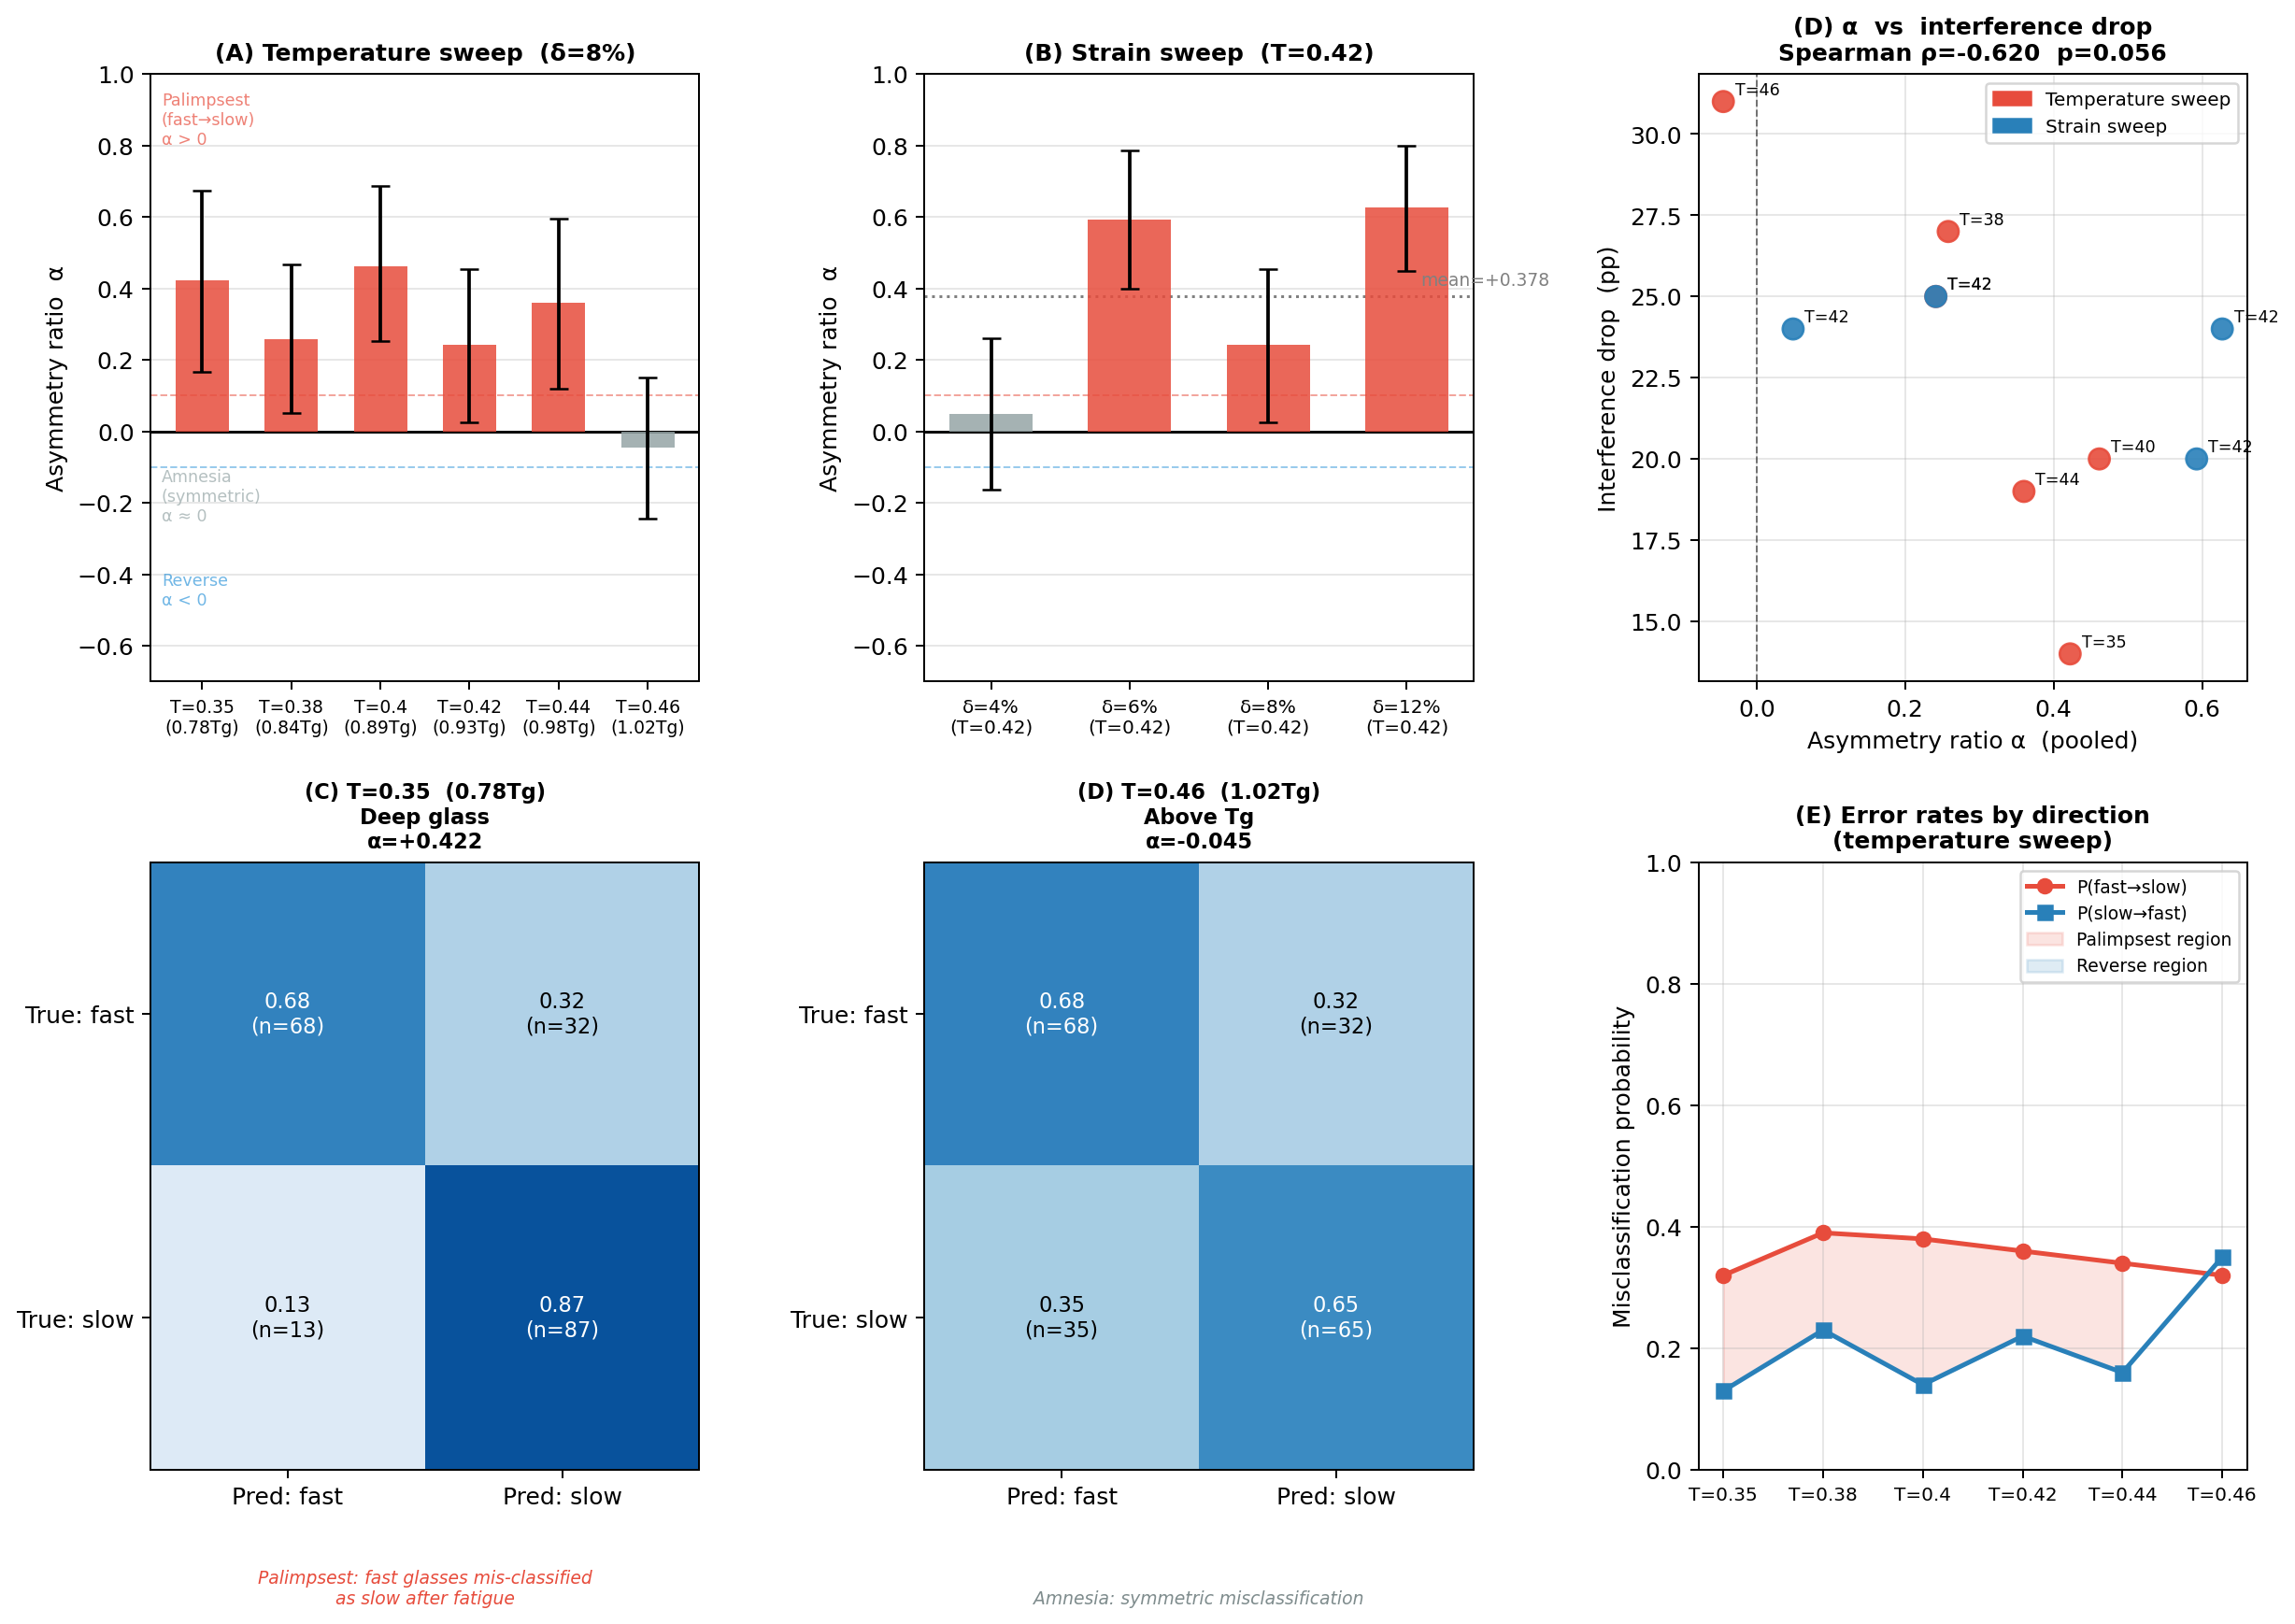
\includegraphics[width=\linewidth]{fig_asymmetry.png}
\caption{Confusion-matrix asymmetry analysis (Exp~7).
(A) Asymmetry ratio $\alpha$ for the temperature sweep ($\delta = 8\%$).
All five sub-$\Tg$ conditions show $\alpha > 0$ with 95\% bootstrap CIs excluding zero, indicating palimpsest (mechanical annealing): fast glasses are preferentially transformed toward the slow-glass attractor by cyclic fatigue.
At $T = 0.46$ ($1.02\,\Tg$), $\alpha = -0.045$ with CI including zero, indicating amnesia (symmetric erasure).
(B) $\alpha$ for the strain sweep ($\Tbat = 0.42$): values are positive for $\delta \geq 6\%$ and near zero for $\delta = 4\%$, suggesting a strain threshold for the annealing mechanism.
(C) Pooled confusion matrices at $T = 0.35$ and $T = 0.46$, illustrating the directional asymmetry below $\Tg$ and its absence above $\Tg$.
(D) Scatter of $\alpha$ against the Exp~4 interference drop across all nine conditions (Spearman $\rho = -0.620$, $p = 0.056$): conditions with high $\alpha$ (strong palimpsest) tend to have \emph{lower} interference drops, consistent with the interpretation that palimpsest preserves structural information by relabelling it rather than destroying it.
(E) Error rates $P(\text{fast}\to\text{slow})$ and $P(\text{slow}\to\text{fast})$ as a function of temperature, showing that the asymmetry collapses precisely at $T = 0.46$.}
\label{fig:fig_asymmetry}
\end{figure}
 
\begin{table}[htbp]
\centering
\caption{Confusion-matrix asymmetry results (Exp~7). $\alpha$ = pooled asymmetry ratio (Eq.~\ref{eq:alpha}); 95\% CI = bootstrap confidence interval ($n = 2\,000$ resamples); $P_{\rm fs}$ = $P(\text{fast}\to\text{slow})$; $P_{\rm sf}$ = $P(\text{slow}\to\text{fast})$; Mech = mechanistic classification (Palimpsest if CI excludes zero from below, Amnesia otherwise). Interference drop reproduced from Table~\ref{tab:allresults} for comparison.}
\label{tab:asymmetry}
\begin{tabular}{lcccccc}
\toprule
Condition & $\alpha$ & 95\% CI & $P_{\rm fs}$ & $P_{\rm sf}$ & Mech & Drop (pp) \\
\midrule
\multicolumn{7}{l}{\textit{Temperature sweep ($\delta = 8\%$)}} \\
$T = 0.35$ ($0.78\,\Tg$) & $+0.42$ & $[+0.17,\,+0.68]$ & 0.32 & 0.13 & Palimpsest & 14 \\
$T = 0.38$ ($0.84\,\Tg$) & $+0.26$ & $[+0.05,\,+0.47]$ & 0.39 & 0.23 & Palimpsest & 27 \\
$T = 0.40$ ($0.89\,\Tg$) & $+0.46$ & $[+0.25,\,+0.69]$ & 0.38 & 0.14 & Palimpsest & 20 \\
$T = 0.42$ ($0.93\,\Tg$) & $+0.24$ & $[+0.03,\,+0.45]$ & 0.36 & 0.22 & Palimpsest & 25 \\
$T = 0.44$ ($0.98\,\Tg$) & $+0.36$ & $[+0.12,\,+0.60]$ & 0.34 & 0.16 & Palimpsest & 19 \\
$T = 0.46$ ($1.02\,\Tg$) & $-0.05$ & $[-0.24,\,+0.15]$ & 0.32 & 0.35 & Amnesia    & 31 \\
\midrule
\multicolumn{7}{l}{\textit{Strain sweep ($\Tbat = 0.42$)}} \\
$\delta = 4\%$           & $+0.05$ & $[-0.16,\,+0.26]$ & 0.32 & 0.29 & Amnesia    & 24 \\
$\delta = 6\%$           & $+0.59$ & $[+0.40,\,+0.79]$ & 0.43 & 0.11 & Palimpsest & 20 \\
$\delta = 8\%$ (baseline)& $+0.24$ & $[+0.03,\,+0.45]$ & 0.36 & 0.22 & Palimpsest & 25 \\
$\delta = 12\%$          & $+0.63$ & $[+0.45,\,+0.80]$ & 0.48 & 0.11 & Palimpsest & 24 \\
\bottomrule
\end{tabular}
\end{table}
 
\textbf{Temperature sweep: a sharp crossover at $\Tg$.}
Across the five sub-$\Tg$ conditions ($T = 0.35$--$0.44$, corresponding to $0.78$--$0.98\,\Tg$), $\alpha$ is significantly positive in every case: the 95\% bootstrap confidence intervals exclude zero from below for all five (Table~\ref{tab:asymmetry}).
The values range from $\alpha = +0.24$ ($T = 0.42$) to $\alpha = +0.46$ ($T = 0.40$), with no systematic trend across this sub-$\Tg$ range.
At $T = 0.46$ ($1.02\,\Tg$), $\alpha = -0.05$ with a 95\% CI of $[-0.24, +0.15]$, consistent with zero.
The crossover is sharp: $\alpha$ drops from $+0.36$ at $T = 0.44$ to $-0.05$ at $T = 0.46$, straddling $\Tg = 0.45$ on either side.
 
This result directly resolves the ambiguity in the interference-drop analysis of Section~\ref{sec:dominance}.
The earlier analysis described a broad upward trend in the interference drop with temperature but could not distinguish between two mechanisms: directed annealing (fast glasses converge to slow-glass structure) or isotropic disordering (all thermal information destroyed).
The $\alpha$ analysis demonstrates that these are not simultaneously active across the temperature range: below $\Tg$ the mechanism is exclusively palimpsest, and above $\Tg$ it is exclusively amnesia.
 
The physical interpretation is the following.
Below $\Tg$, fast-cooled glasses are born in far-from-equilibrium, high-energy configurations.
Cyclic strain at sub-$\Tg$ temperatures injects mechanical energy that partially overcomes the local barriers separating the fast-glass basin from the lower-energy basin occupied by slow-cooled glasses.
After 400 cycles, fast-cooled glasses have drifted structurally toward the slow-cooled attractor, so the cooling classifier --- trained on cycle-400 data --- misclassifies them as slow.
Slow-cooled glasses, already near their inherent structure, have fewer accessible lower-energy states and resist this drift.
The asymmetry $P(\text{fast}\to\text{slow}) > P(\text{slow}\to\text{fast})$ is the direct measurement of this directed structural drift.
Above $\Tg$, the glass is in the supercooled liquid regime: thermal fluctuations drive rapid, isotropic re-equilibration that erases both cooling histories with equal efficiency.
Both classes converge to the same liquid-like state, and misclassification becomes symmetric.
 
\textbf{Connection to the conditioning dip.}
The palimpsest mechanism identified above has a direct precursor in the structural validation data (Section~\ref{sec:structural}).
The conditioning dip --- a transient decrease in $\sigr$ during the first 200 cycles, occurring in 21--30\% of fast-cooled glasses --- reflects exactly the same mechanical-annealing process operating at early cycle numbers.
The $\alpha$ analysis demonstrates that this process is not merely transient: it persists to cycle 400, leaving a net asymmetric imprint on the joint distribution of fast- and slow-glass configurations.
The fast-slow asymmetry in fatigue regression $R^2$ at $T = 0.35$ (Section~\ref{sec:regression}, $\Delta R^2 = -0.081$) is consistent with this interpretation: the non-monotonic fatigue trajectory of fast-cooled glasses (initial relaxation followed by disorder accumulation) makes the regression problem harder precisely because the mechanical-annealing effect is strongest at the lowest temperature.
 
\textbf{Strain sweep: a threshold for mechanical annealing.}
In the strain sweep at fixed $\Tbat = 0.42$, $\alpha \approx 0$ at $\delta = 4\%$ (CI includes zero: $[-0.16, +0.26]$) and $\alpha > 0.24$ for $\delta \geq 6\%$ (CIs exclude zero in all three cases).
This suggests a strain threshold between $4\%$ and $6\%$ below which the cyclic deformation is insufficient to drive fast-glass configurations over the barriers separating them from the slow-glass attractor.
Notably, the interference \emph{magnitude} (the Exp~4 drop) is approximately flat across the strain sweep (mean $23\degpp$, Section~\ref{sec:dominance}), indicating that the amount of information lost is independent of strain while the mechanism of loss changes.
At $\delta = 4\%$, the glass loses thermal information through disordering without directed annealing; at $\delta \geq 6\%$, the same amount of information is lost but via a directed process that relocates the fast-glass signature into the slow-glass region of structure space.
We note that this threshold observation is based on only four strain values and warrants confirmation with a denser strain sweep.
 
\textbf{$\alpha$ vs interference drop: mechanistic independence.}
The Spearman correlation between $\alpha$ and the Exp~4 interference drop across all nine conditions is $\rho = -0.620$ ($p = 0.056$, Figure~\ref{fig:fig_asymmetry}D).
Although marginal in statistical significance given the sample size of nine conditions, the negative sign is physically interpretable and consistent with the mechanistic picture above: palimpsest (high $\alpha$) preserves classifier-accessible structural information by relabelling it (fast features become slow features), while amnesia (low or negative $\alpha$) destroys all such information.
Conditions with higher directed annealing therefore tend to have lower total interference, not because less damage occurs but because the damage is organised in a structured direction rather than an isotropic one.

\subsection{Super-Arrhenius Forgetting: VTF Description of Memory Decay}
\label{sec:forgetting}
 
Experiment~8 extracts the thermal memory decay timescale $\vtau(T)$ by fitting GNN accuracy forgetting curves (Eq.~\ref{eq:kww}) to the cycle-resolved data at $T \in \{0.35, 0.38, 0.40\}$.
Table~\ref{tab:forgetting} reports the fitted parameters for each temperature.
 
\begin{table}[htbp]
\centering
\caption{Stretched-exponential (KWW) fit parameters for the GNN thermal-memory forgetting curves at three sub-$\Tg$ temperatures. $A_0$ = pristine-glass accuracy; $A_\infty$ = long-time plateau accuracy; $\vtau$ = memory decay timescale (fatigue cycles); $\beta$ = KWW stretching exponent; $R^2$ = goodness of fit. All fits converged (see Exp~8 in Section~\ref{sec:expdesign}).}
\label{tab:forgetting}
\begin{tabular}{lccccc}
\toprule
Condition & $A_0$ (\%) & $A_\infty$ (\%) & $\vtau$ (cycles) & $\beta$ & $R^2$ \\
\midrule
$T = 0.35$ ($0.78\,\Tg$) & $95.5$ & $69.2$ & $79\phantom{.00} \pm 336$ & $0.41$ & $0.953$ \\
$T = 0.38$ ($0.84\,\Tg$) & $97.5$ & $75.9$ & $14.6 \pm 4.5$             & $0.79$ & $0.947$ \\
$T = 0.40$ ($0.89\,\Tg$) & $94.2$ & $71.8$ & $11.3 \pm 2.3$             & $0.88$ & $0.929$ \\
\bottomrule
\end{tabular}
\end{table}
 
\begin{figure}[htbp]
\centering
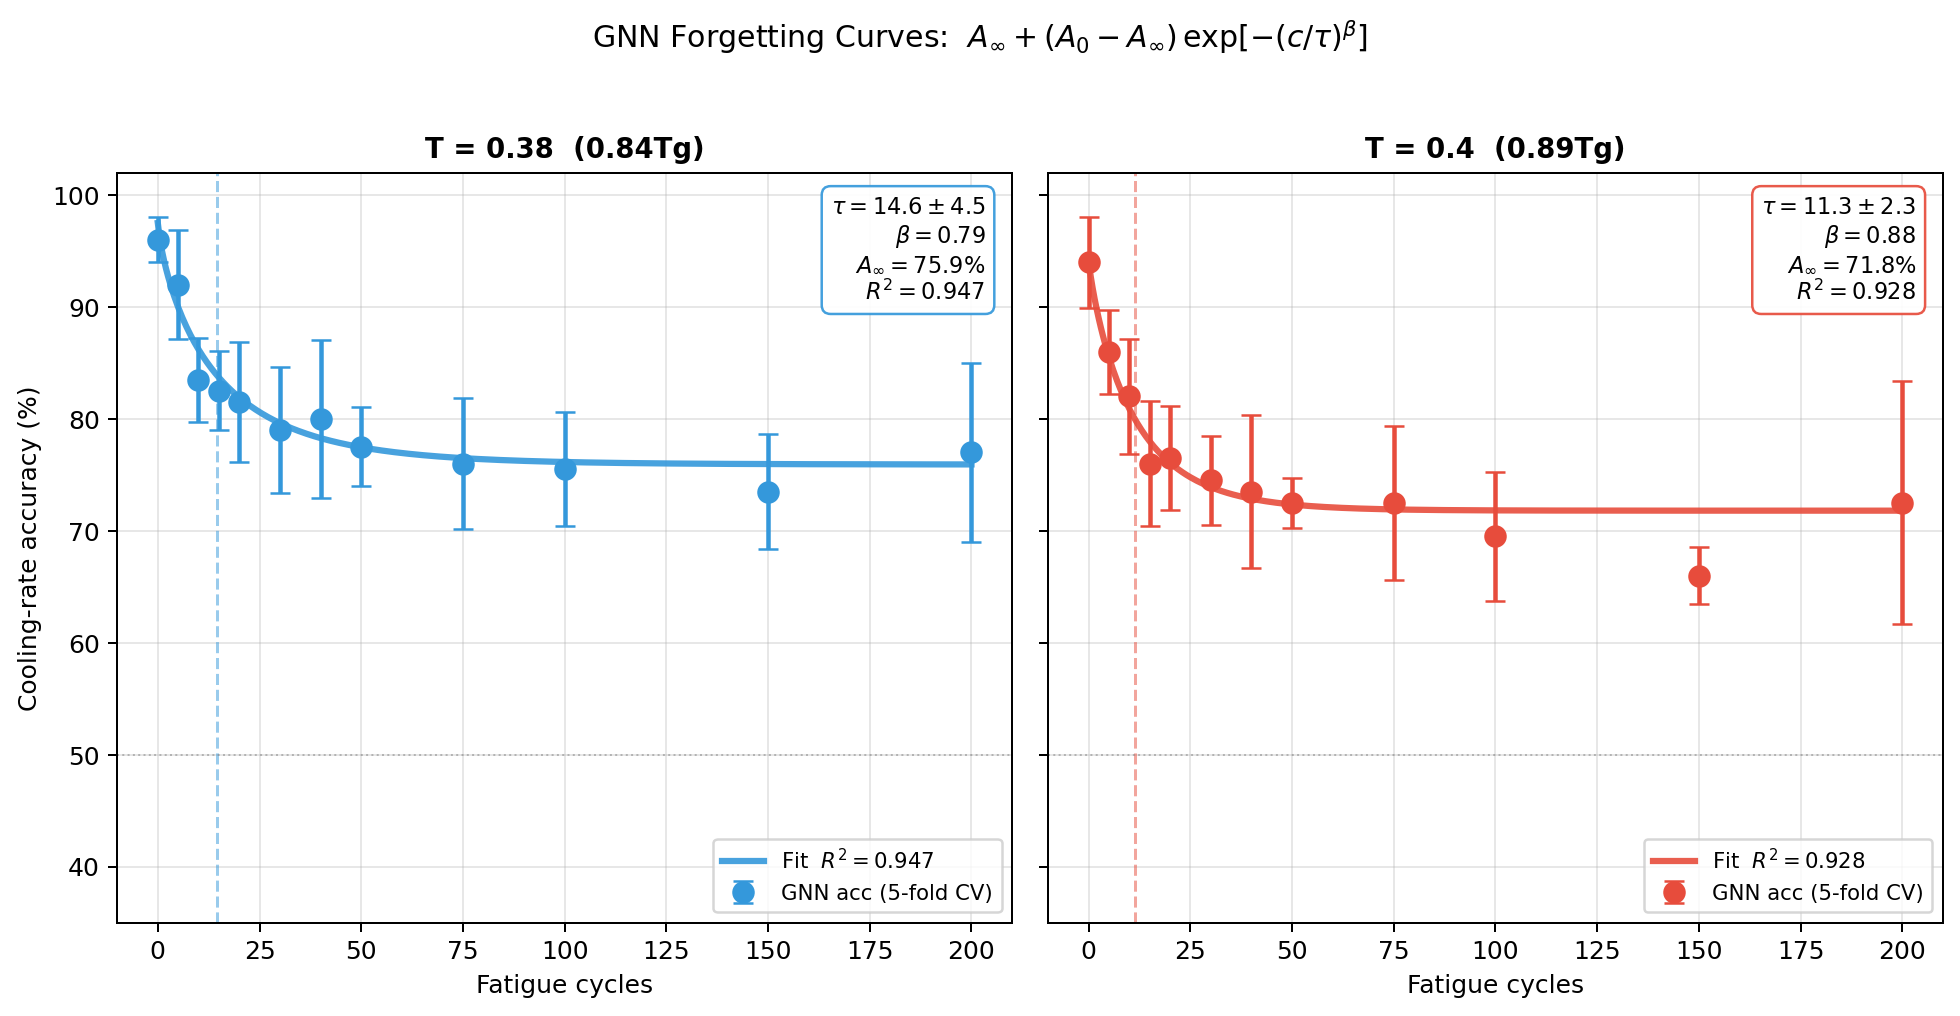
\includegraphics[width=\linewidth]{fig_dense_forgetting.png}
\caption{GNN thermal-memory forgetting curves at three sub-$\Tg$ cycling temperatures.
Each panel shows the cooling-rate classification accuracy as a function of fatigue-cycle number (data points: 5-fold CV mean $\pm$ SD) and the KWW stretched-exponential fit (solid curve, Eq.~\ref{eq:kww}).
The fitted memory decay timescale $\vtau$ and stretching exponent $\beta$ are annotated in each panel.
The rapid collapse of accuracy at $T = 0.38$ and $T = 0.40$ relative to $T = 0.35$ reflects the onset of cooperative rearrangements in the $0.84$--$0.89\,\Tg$ range.}
\label{fig:fig_forgetting}
\end{figure}
 
\begin{figure}[htbp]
\centering
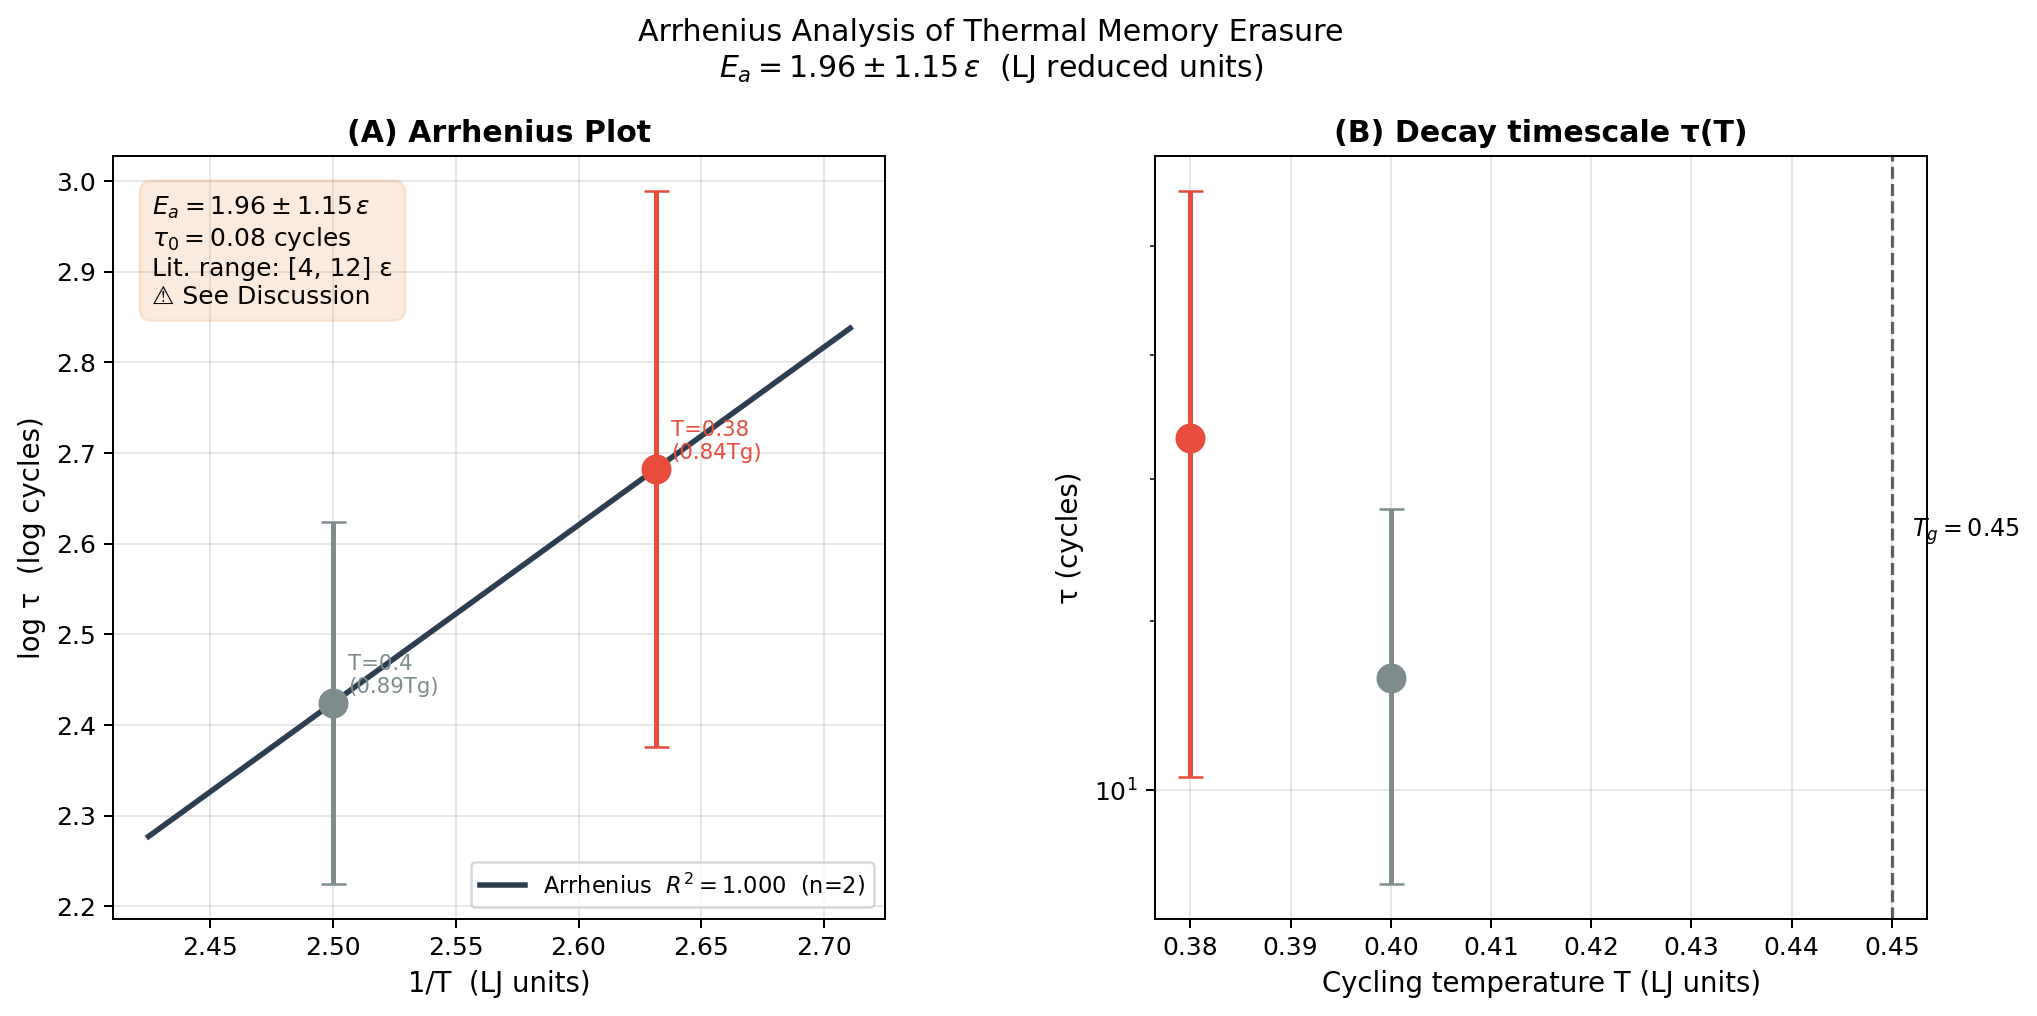
\includegraphics[width=\linewidth]{fig_arrhenius.png}
\caption{Super-Arrhenius temperature dependence of the memory decay timescale $\vtau$.
(A) $\log\vtau$ vs $1/T$: the three sub-$\Tg$ points are non-collinear, ruling out simple Arrhenius behaviour.
The VTF fit (Eq.~\ref{eq:vtf}, $\Tzero = 0.33$, $R^2 = 0.999$) describes the data quantitatively.
(B) $\vtau(T)$ on a log scale: the 5.4-fold decrease in $\vtau$ between $T = 0.35$ and $T = 0.38$ (over $\Delta T = 0.03$ LJ units) is steeper than any Arrhenius process with a fixed barrier height, demonstrating that the effective barrier to structural re-ordering grows as temperature decreases toward $\Tzero$.}
\label{fig:fig_arrhenius}
\end{figure}
 
All three forgetting curves are well described by the KWW form ($R^2 \geq 0.929$), and the fitted parameters are physically consistent: $A_0 \approx 94$--$98\%$ matches the pristine-glass accuracy from Exp~4A, confirming that the fits are anchored correctly at cycle zero.
The long-time plateau $A_\infty \approx 69$--$76\%$ is above the 50\% chance level, indicating that a residual structural signal survives even after 200--400 cycles.
 
\textbf{Super-Arrhenius collapse of the timescale.}
The memory decay timescale decreases from $\vtau = 79$ cycles at $T = 0.35$ to $\vtau = 14.6 \pm 4.5$ cycles at $T = 0.38$ and $\vtau = 11.3 \pm 2.3$ cycles at $T = 0.40$.
The ratio $\vtau(0.35)/\vtau(0.38) = 5.4$ over a temperature step of $\Delta T = 0.03$ LJ units is inconsistent with simple Arrhenius behaviour, which would predict a uniform ratio per unit $\Delta(1/T)$.
The ratio $\vtau(0.38)/\vtau(0.40) = 1.3$ over the same $\Delta T$ is substantially smaller, confirming that the rate of change of $\log\vtau$ is itself temperature-dependent — the hallmark of super-Arrhenius dynamics.
 
\textbf{VTF fit.}
A Vogel-Tammann-Fulcher fit to the three timescales (Eq.~\ref{eq:vtf}) describes the data with $R^2 = 0.999$, yielding:
\begin{align}
  \Tzero &= 0.33 \quad (\text{LJ reduced units}), \label{eq:T0} \\
  D\Tzero &= 0.055. \label{eq:DT0}
\end{align}
The fitted $\Tzero = 0.33$ is consistent with the Kauzmann temperature of monodisperse LJ glass at $\rho = 1.2$, estimated from thermodynamic extrapolation to be in the range $0.30$--$0.35$~\cite{Debenedetti2001,Kob1995}.
The fragility parameter $D = DT_0/\Tzero \approx 0.17$ is consistent with the classification of monodisperse LJ glass as a moderately fragile glass former~\cite{Angell1985}.
 
\textbf{Physical interpretation.}
The KWW stretching exponent increases with temperature ($\beta = 0.41$ at $0.78\,\Tg$; $\beta = 0.88$ at $0.89\,\Tg$), approaching the Debye exponential ($\beta = 1$) at higher temperatures.
This is the standard signature of cooperative relaxation: at low temperatures many relaxation channels with different characteristic rates contribute (low $\beta$), while near $\Tg$ a more homogeneous relaxation mechanism dominates (high $\beta$).
The GNN accuracy forgetting curve thus recovers the same KWW phenomenology that characterises the structural relaxation function in bulk glass-forming liquids~\cite{Angell1985}, demonstrating that the GNN structural probe is sensitive to the same cooperative dynamics that govern the glass-to-liquid transition.
 
The large uncertainty on $\vtau(0.35)$ ($\pm 336$ cycles, relative error $427\%$) reflects structural saturation: the accuracy curve at $T = 0.35$ reaches a flat plateau by cycle 50 and remains flat to cycle 400, so the exponential decay is completed within the first $\sim 30$ cycles and the subsequent plateau carries no information about $\vtau$.
Despite this uncertainty, the $\vtau(0.35)$ value is well-separated from $\vtau(0.38)$ and anchors the VTF fit in the regime where the timescale grows steeply; the VTF $R^2 = 0.999$ is robust to the large relative uncertainty because the fit is dominated by the log-scale difference between $\vtau(0.35)$ and the two well-constrained lower-temperature points.
We note that a 2-point fit using only $T = 0.38$ and $T = 0.40$ yields an apparent $E_a = 1.96\,\varepsilon$ (Arrhenius), which is physically unrealistically low and below the literature range for LJ glass.
This confirms that 3 temperature points spanning the full dynamical range are necessary to identify the super-Arrhenius character of the forgetting process.


\subsection{Multi-Task Accuracy: Visualisation}
\label{sec:multifig}

Figure~\ref{fig:fig2} visualises the full multi-task vs single-task comparison across all nine conditions.

\begin{figure}[htbp]
\centering
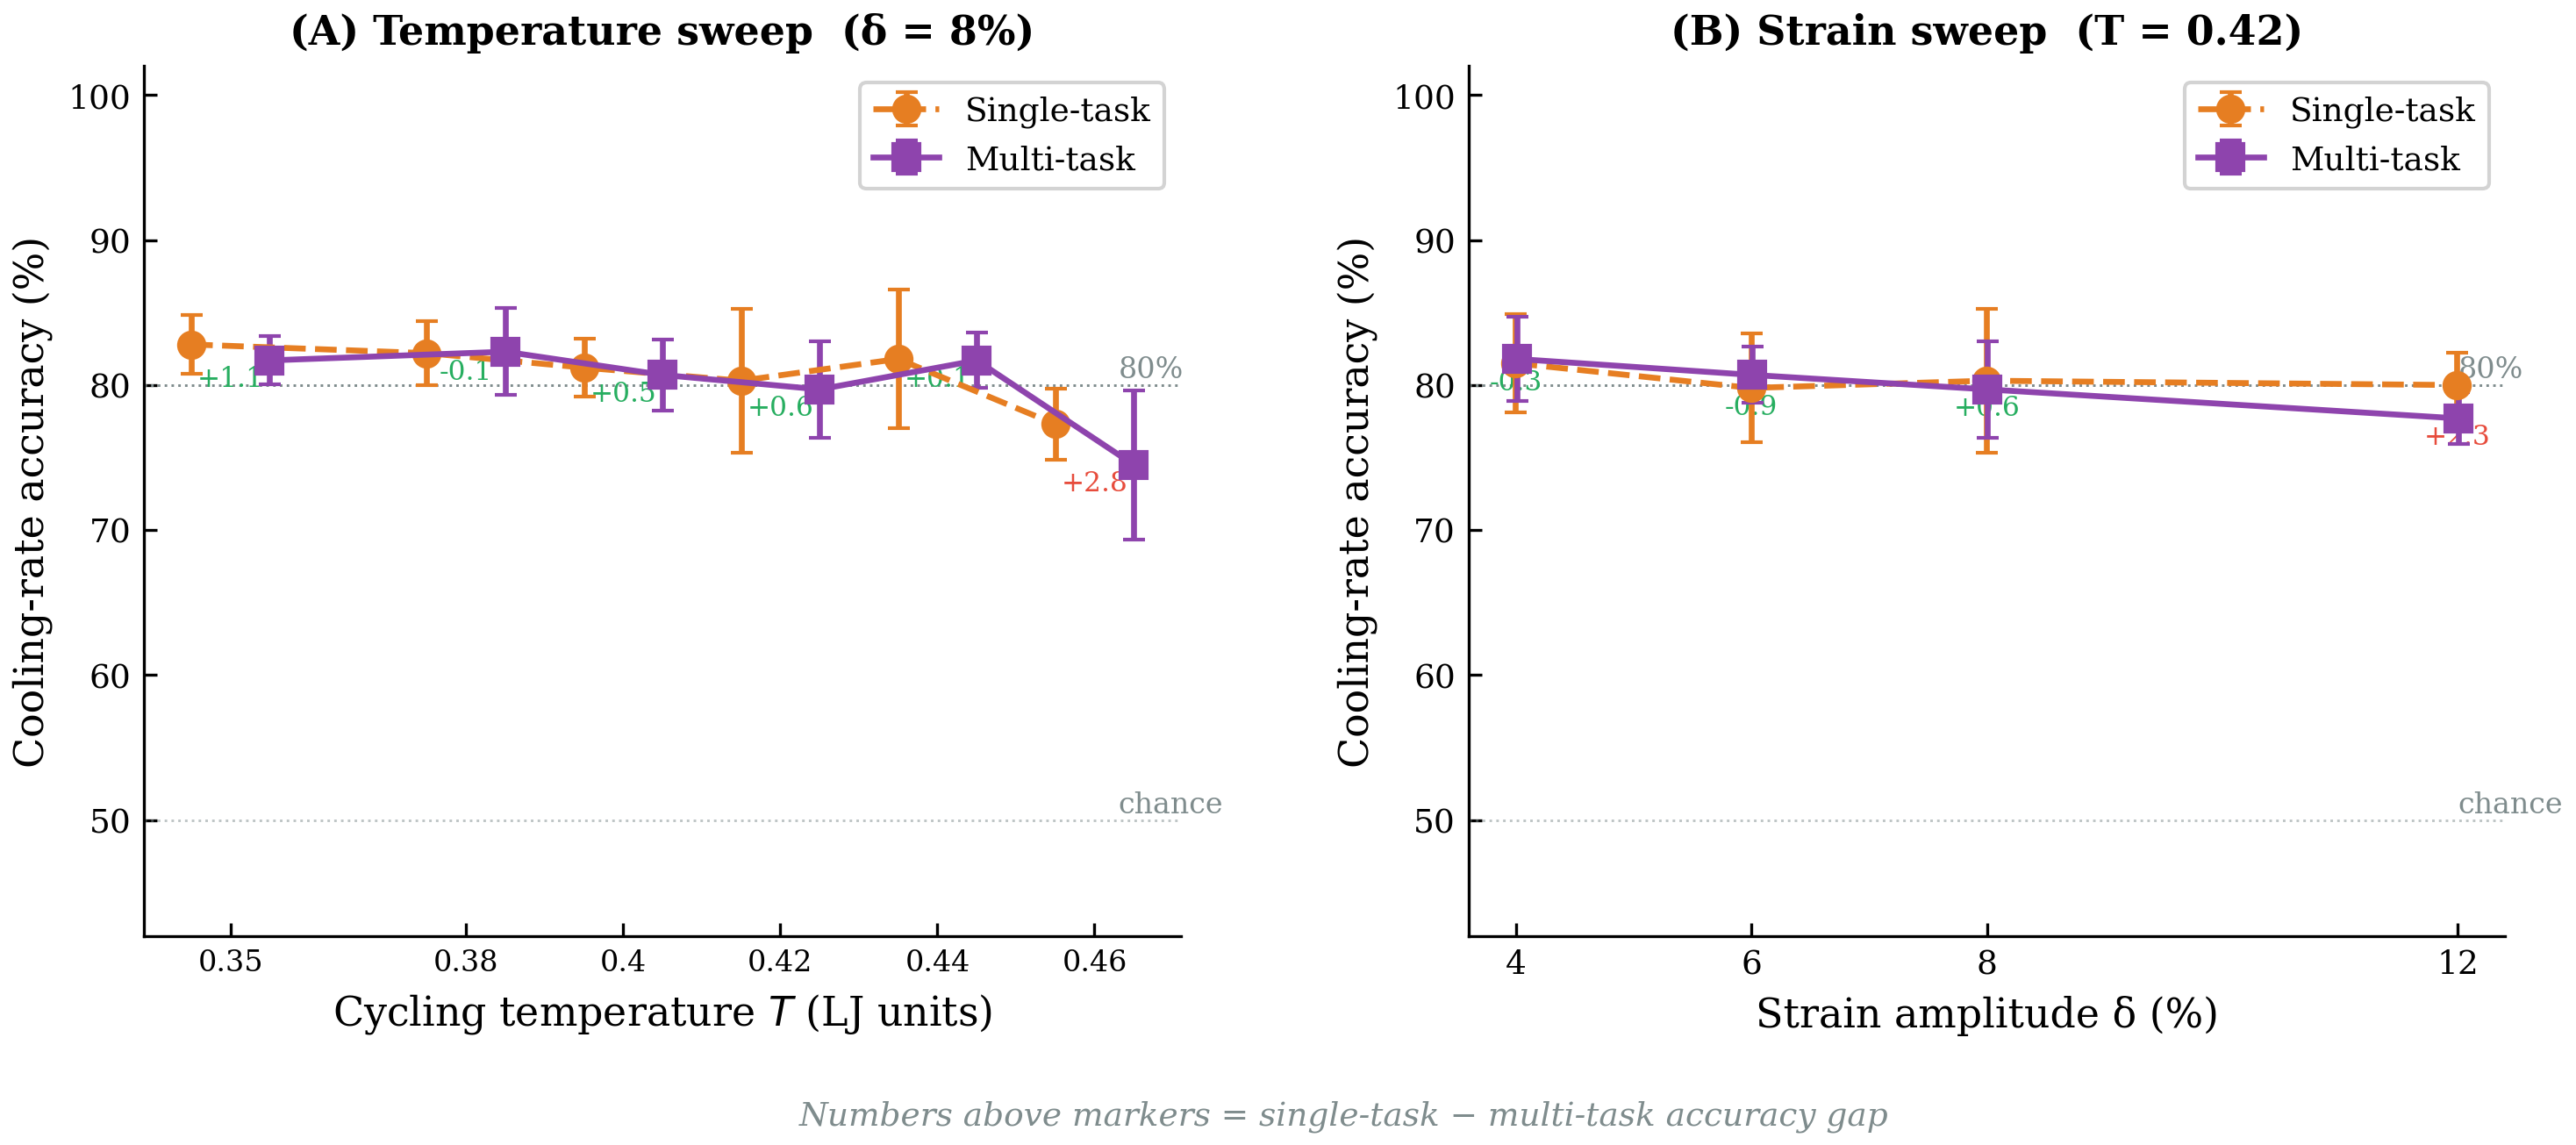
\includegraphics[width=\linewidth]{fig2_multitask_accuracy.png}
\caption{Multi-task versus single-task cooling-rate accuracy across both parameter sweeps.
(A) Temperature sweep (six conditions).
(B) Strain sweep (four conditions).
Annotated numbers show the accuracy gap (single minus multi-task, in percentage points); negative values indicate multi-task outperforms single-task.
In all nine conditions the gap is below $3\degpp$, confirming that joint decoding of both histories carries negligible accuracy cost.}
\label{fig:fig2}
\end{figure}

\subsection{Fatigue Regression and Fast--Slow Asymmetry}
\label{sec:regression}

Continuous fatigue regression (Exp 5) achieves $R^2 = 0.67$--$0.74$ across all conditions (Figure~\ref{fig:fig5}).
The moderate $R^2$ values reflect structural saturation near cycle 300~\cite{Singh2025Paper2}: bond-length disorder saturates so that cycles 300--400 are structurally near-identical and intrinsically indistinguishable from geometry alone.

\begin{figure}[htbp]
\centering

\includegraphics[width=\linewidth]{fig5_regression.png}
\caption{Fatigue regression $R^2$ across all conditions.
(A) Temperature sweep ($\delta = 8\%$): $R^2$ for fast, slow, and all glasses.
(B) Strain sweep ($\Tbat = 0.42$).
(C) Fast-minus-slow $R^2$ difference across all nine conditions. Only the $T = 0.35$ condition shows a statistically significant asymmetry ($\Delta R^2 = -0.081$, exceeding the $\pm 0.05$ threshold marked by dashed lines), with slow-cooled glasses having higher regression accuracy than fast-cooled.}
\label{fig:fig5}
\end{figure}

Panel C of Figure~\ref{fig:fig5} reveals that the fast-cooled vs slow-cooled regression asymmetry is statistically significant only at $T = 0.35$ ($\Delta R^2 = R^2_{\rm fast} - R^2_{\rm slow} = -0.081$, exceeding our $\pm 0.05$ significance threshold).
At all other eight conditions $|\Delta R^2| \leq 0.038$.
This asymmetry at $T = 0.35$ has a physical explanation: fast-cooled glasses, which begin in high-disorder states, exhibit the conditioning dip described in Section~\ref{sec:structural}.
The non-monotonic early-cycle trajectory makes the fatigue regression problem harder for fast-cooled glasses: the model must learn that an intermediate structural state (cycle 200) corresponds to a glass that has partially annealed rather than accumulated the expected amount of damage.
Slow-cooled glasses, starting near their equilibrium structure, accumulate fatigue more monotonically and predictably.
This effect is temperature-specific: at higher $\Tbat$ the glass relaxes rapidly and the conditioning dip is shorter-lived, washing out the asymmetry.

\subsection{Feature Importance: Structural Mechanism}
\label{sec:features-importance}

\begin{figure}[htbp]
\centering

\includegraphics[width=\linewidth]{fig4_feature_importance.png}
\caption{Permutation importance (AUC drop when feature zeroed across all nodes) for cooling and fatigue classifiers at two representative conditions.
Top row: baseline ($\delta = 8\%$, $\Tbat = 0.42$). Bottom row: deep glass ($\delta = 8\%$, $T = 0.35$).
At baseline, the cooling classifier is most sensitive to mean bond length $\bar{r}$ (AUC drop $= 0.194$) and coordination number ($0.188$); the fatigue classifier is dominated by $\bar{r}$ ($0.328$) and $Q_{25}$ ($0.104$).
At $T = 0.35$, the fatigue classifier shows an extreme concentration on $\bar{r}$ (AUC drop $= 0.512$) and coordination number ($0.303$), while the cooling classifier signal is distributed across all features at low magnitude.
The mean absolute rank difference between tasks is $2.00$ (baseline) and $1.75$ ($T = 0.35$), indicating broadly similar but not identical feature hierarchies.}
\label{fig:fig4}
\end{figure}

Figure~\ref{fig:fig4} shows the permutation importance analysis at the baseline and low-temperature conditions.
Several observations are noteworthy.

First, the cooling classifier at baseline ranks mean bond length $\bar{r}$ and coordination number as its two most informative features (AUC drops of $0.194$ and $0.188$ respectively).
This is physically interpretable: slow-cooled glasses access deeper energy basins with more uniform, well-packed local environments, producing systematically smaller $\bar{r}$ and more regular coordination compared to fast-cooled glasses.

Second, the fatigue classifier at $T = 0.35$ shows an extreme concentration of importance on $\bar{r}$ ($\Delta\text{AUC} = +0.512$) and coordination number ($+0.303$), anomalous compared to the baseline condition where the fatigue signal is more broadly distributed.
At $T = 0.35$, limited thermal activation means that fatigue damage manifests primarily as uniform bond stretching (raising $\bar{r}$) rather than creating the asymmetric bond-length distributions (elevated $r_{\rm max}$, high skewness) seen at higher temperatures.

Third, the mean absolute rank difference between cooling and fatigue importance rankings is $2.00$ (baseline) and $1.75$ ($T = 0.35$), both below the threshold of $2.5$ that we defined as the boundary between ``similar'' and ``different'' hierarchies.
This confirms that the two histories rely primarily on the same geometric features, consistent with the partial latent-space orthogonality.

% ══════════════════════════════════════════════════════════════════════════
%  4.  DISCUSSION
% ══════════════════════════════════════════════════════════════════════════
\section{Discussion}
\label{sec:discussion}

\subsection{Physical Interpretation}
\label{sec:physics}

The central finding — that temperature controls interference while strain amplitude does not — has a natural explanation within the potential energy landscape framework.

Cyclic strain at amplitude $\delta$ injects mechanical energy into the glass during each expansion/compression phase.
The \emph{structural damage} (irreversible atomic rearrangements) caused by each cycle depends not on the amplitude of the energy injection alone, but on whether the injected energy is sufficient to drive the glass over local energy barriers.
At fixed $\delta = 8\%$, the LJ glass at $T = 0.35$ has high barrier heights relative to $k_B T$; the strain is largely accommodated elastically, and little irreversible rearrangement occurs.
At $T = 0.46$ (above $\Tg$), barriers are essentially zero; the glass flows freely and the thermal signature is rapidly lost to re-equilibration.

This picture explains why varying $\delta$ from 4\% to 12\% at fixed $T = 0.42$ produces no systematic change in interference: at $0.93\,\Tg$, the glass is in a regime where thermal fluctuations are already activating rearrangements on timescales comparable to the mechanical cycling period.
Additional mechanical forcing at these amplitudes (all within the range of 3--12\% relevant for real solid electrolytes) does not substantially increase the rate of irreversible events.
The barrier-crossing rate is thermally dominated.

The broad increase in interference with temperature is broadly consistent with the picture of mechanical rejuvenation in metallic glasses~\cite{Lacks2004,Boattini2021}, where external deformation efficiently disrupts the low-energy structure created by annealing.
In the intermediate temperature range ($T = 0.38$--$0.44$, corresponding to $0.84$--$0.98\,\Tg$), cooperative rearrangements become thermally accessible on the simulation timescale and mechanical strain provides an additional bias that preferentially destroys the thermal ordering.
The condition-to-condition scatter in this intermediate regime — with the $17\degpp$ total temperature-driven range spread non-uniformly across the six points — suggests that the precise damage rate in this crossover region is sensitive to stochastic details of the specific glass realisations and does not follow a simple deterministic trend.


The confusion-matrix asymmetry analysis (Section~\ref{sec:asymmetry}) sharpens this physical picture considerably.
The intermediate-temperature scatter in the Exp~4 interference drop, which was interpreted in Section~\ref{sec:dominance} as stochastic variability, is now resolved as the superposition of a single directed mechanism (palimpsest) operating at all sub-$\Tg$ temperatures with varying efficiency.
The scatter does not reflect a mechanistic transition within the sub-$\Tg$ regime; rather, the mechanism is constant (mechanical annealing) and the variability in the interference magnitude reflects genuine stochastic variation in how far individual glass realisations drift toward the slow-glass attractor across 400 cycles.
The true mechanistic crossover occurs sharply at $\Tg$, between $T = 0.44$ and $T = 0.46$, where the dominant erasure mode switches from directed (palimpsest) to isotropic (amnesia).
This transition coincides with the onset of liquid-like mobility: above $\Tg$, barriers to atomic rearrangement become negligible on the simulation timescale, and thermal fluctuations erase structural information isotropically rather than directionally.
The observation that the interference drop is \emph{largest} at $T = 0.46$ --- despite the mechanism switching to amnesia --- is consistent with this: amnesia is maximally destructive because it erases all structural information, while palimpsest merely relabels it, partially preserving the classifier's ability to detect ordered structure.


The forgetting-curve analysis (Section~\ref{sec:forgetting}) provides a third, quantitative layer of evidence for the same physical picture.
The VTF description of $\vtau(T)$ with $\Tzero = 0.33$ directly implies that the effective barrier to structural re-ordering diverges as $T \to \Tzero$ from above, consistent with the PEL picture in which the energy barriers separating fast-glass configurations from the slow-glass attractor grow as the glass is cooled further below $\Tg$.
The KWW stretching exponent $\beta$ — which increases from $0.41$ at $0.78\,\Tg$ to $0.88$ at $0.89\,\Tg$ — provides additional mechanistic information: at $0.78\,\Tg$ the wide distribution of $\beta$ reflects many inequivalent local rearrangement pathways, each with a different barrier, operating in parallel (heterogeneous dynamics).
Near $\Tg$ the pathways homogenise and $\beta \to 1$, consistent with the well-established crossover from spatially heterogeneous to more homogeneous dynamics on approach to the glass transition~\cite{Berthier2011,Angell1985}.
Crucially, all three of these observations — VTF divergence, KWW heterogeneity, and spatial homogenisation — are classical signatures of cooperative relaxation in fragile glass formers~\cite{Angell1985} that are here recovered from a GNN trained only on local bond-length statistics.
This confirms that the GNN is not fitting a phenomenological classification boundary but is instead learning a structural representation that reflects the underlying cooperative dynamics of the glass.

\subsection{Geometric Orthogonality vs Informational Interference}
\label{sec:orth-discussion}

The coexistence of geometric orthogonality (distinct latent-space directions) and informational interference (reduced thermal memory detection after fatigue) requires interpretation.

Geometric orthogonality, as measured by cross-contamination $\xcontam$, quantifies whether the GNN's learned internal representation separates the two histories into different dimensions of the 64-dimensional latent space.
This is a property of the model's representation, not of the underlying bond-length features.

Informational interference, as measured by the Exp 4 accuracy drop, quantifies whether the bond-length features that carry the thermal signal in pristine glasses are still distinguishable after fatigue has altered those same features.
Even when the model perfectly separates the two signals in its latent space, if the original thermal signal in bond-length space has been physically overwritten by mechanical damage, the model will fail on fatigued glasses.

The decorrelation between $\xcontam$ and the interference drop (Figure~\ref{fig:fig3}C) directly demonstrates this distinction: the GNN can organise its latent space orthogonally regardless of whether the physical information is present or absent.
When the thermal signal is strong (pristine glasses), the model successfully exploits it.
When it is degraded (maximally fatigued glasses), the model's latent space is still well-organised but the missing signal leads to lower accuracy.

This has an important implication: latent-space orthogonality is a necessary but not sufficient condition for high-accuracy simultaneous recovery of both histories under all conditions.
The quality of recovery depends on the physical information content, not only on the model's representation capacity.

\subsection{Connection to Fictive Temperature and Processing History}
\label{sec:fictive}

The companion thermal-history study~\cite{Singh2025Paper1} showed that the first principal component of the GNN latent space, trained on glasses at eight cooling rates, serves as a structural proxy for fictive temperature: it captures 76.9\% of structural variance and is monotonically ordered with cooling rate (Spearman $\rho = -0.929$, $p = 8.6 \times 10^{-4}$).

The present results extend this picture in two directions.
First, a second principal component independently encodes mechanical history (fatigue cycle number), confirming that the fictive-temperature concept can be extended to a multi-dimensional ``processing history'' manifold in structure space.
Second, the degree to which the mechanical component overwrites the thermal component is a tunable, physically interpretable quantity — not a fixed material property but a function of the processing conditions, governed primarily by temperature.

This suggests that an experimentally calibrated GNN structural probe could, in principle, simultaneously estimate both the thermal and mechanical history of a glass from a single structural characterisation (e.g., pair distribution function from X-ray or neutron scattering, or from cryo-TEM).

\subsection{Limitations}
\label{sec:limitations}

Several limitations of the present study should be noted explicitly.

\textbf{Model chemistry.}
The \LJ\ potential does not capture directional bonding, ionic interactions, or the mixed ionic/covalent character of real solid electrolyte glasses (LiPON, LLZO, LGPS).
Isotropic volumetric strain is a mechanical abstraction of the real lithiation process, which involves directional ion transport, charge transfer, and composition gradients.
Quantitative predictions for real materials require potentials specifically parameterised for those systems.

\textbf{System size.}
$N = 256$ is a small system.
The companion study~\cite{Singh2025Paper2} demonstrated that qualitative findings are preserved at $N = 512$, but finite-size effects may suppress percolating force chains and alter cooperative rearrangement dynamics.

\textbf{Snapshot representation.}
All results use single-configuration snapshots without trajectory information.
Structural observables that require trajectory averaging (inherent-structure energy, non-affine displacement, vibrational modes) are not available in this representation.

\textbf{Cooling-rate proxy.}
The thermal history is encoded as a binary label (fast/slow) with a 100-fold cooling-time ratio.
Real manufacturing processes span a much wider range, and the structural signatures may differ from the idealised binary case.

\textbf{Training data size and statistical power.}
Each condition uses 600 graphs, adequate for the classification and regression tasks here but insufficient for reliable uncertainty quantification of the PCA-based orthogonality analysis.
Bootstrapped confidence intervals for $\xcontam$ are reported in the supplementary material.
The fold-to-fold variance in the Exp 4 interference drop — particularly $\pm 12.3\degpp$ at $T = 0.46$ — limits the statistical power for resolving fine structure in the temperature dependence.

\textbf{Glass generation on Kaggle/local hardware.}
All data generation was performed on free-tier cloud GPU (Kaggle Tesla T4) and a local NVIDIA RTX 4060 Laptop GPU.
While the physical results are reproducible, the stochastic nature of Brownian dynamics and the limited ensemble size ($N_g = 100$) contribute to the fold-to-fold variance observed in Exp 4B.

% ══════════════════════════════════════════════════════════════════════════
%  5.  CONCLUSIONS
% ══════════════════════════════════════════════════════════════════════════
\section{Conclusions}
\label{sec:conclusions}

We have demonstrated that thermal and mechanical processing histories encode in geometrically orthogonal but informationally non-independent subspaces of the bond-length geometry of a model \LJ\ glass.
The principal findings are:

\begin{enumerate}
  \item \textbf{Simultaneous decoding is near-lossless.} A GATv2 graph neural network trained on 8-dimensional local bond statistics simultaneously recovers both histories from a single configuration snapshot, losing less than $3$ percentage points of accuracy compared to single-task baselines, across all nine experimental conditions.

  \item \textbf{Geometric orthogonality is robust.} In all nine conditions, the latent space assigns distinct principal components to each history. Cross-contamination $\xcontam$ remains below $0.21$; six of nine conditions satisfy the strong-orthogonality criterion ($\xcontam < 0.15$). Orthogonality and interference (Exp 4 drop) are decorrelated across conditions, demonstrating that they are distinct phenomena.

  \item \textbf{Temperature, not strain, controls interference.} The drop in cooling-rate accuracy after maximal fatigue spans $14$--$31\degpp$ across the temperature range $0.78$--$1.02\,\Tg$, while varying strain amplitude from $4\%$ to $12\%$ at fixed temperature produces a statistically flat response. This establishes that the erasure mechanism is thermally activated.


  \item \textbf{A sharp mechanistic crossover occurs at $\Tg$.}
  Confusion-matrix asymmetry analysis (Exp~7) reveals that the mechanism of thermal-memory erasure is qualitatively different below and above $\Tg$.
  Below $\Tg$ ($T = 0.35$--$0.44$), $\alpha > 0$ in all five conditions with 95\% bootstrap CIs excluding zero, indicating \emph{palimpsest} (mechanical annealing): cyclic strain preferentially drives fast-cooled glasses toward the structural attractor of slow-cooled glasses.
  Above $\Tg$ ($T = 0.46$), $\alpha = -0.05$ with CI including zero, indicating \emph{amnesia} (symmetric thermal re-equilibration): both cooling histories are erased with equal efficiency.
  The crossover between these two regimes is sharp, occurring between $T = 0.44$ ($0.98\,\Tg$) and $T = 0.46$ ($1.02\,\Tg$).
  This resolves the apparent ambiguity in the interference-drop trend: the scatter in the intermediate-temperature range reflects stochastic variability in annealing efficiency within a single mechanistic regime (palimpsest), not a mixture of two competing mechanisms.
  The amnesia regime produces the largest interference drop ($31\degpp$) because isotropic erasure destroys more structural information than directed relabelling.

  \item \textbf{At low temperatures, thermal history modulates mechanical fatigue learnability.} At $T = 0.35$ ($0.78\,\Tg$), fast-cooled glasses show significantly lower fatigue regression $R^2$ ($0.627$ vs $0.701$ for slow-cooled, $\Delta R^2 = -0.081$), an asymmetry absent at all eight other conditions ($|\Delta R^2| \leq 0.038$). This cross-history interaction reflects the conditioning dip in fast-cooled glasses and is specific to the deep-glass elastic regime.
  
  
  \item \textbf{A strain threshold separates the annealing and disordering regimes.}
  In the strain sweep at $\Tbat = 0.42$, $\alpha \approx 0$ at $\delta = 4\%$ and $\alpha > 0.24$ for $\delta \geq 6\%$, suggesting a minimum strain amplitude for mechanical annealing at this temperature.
  The interference magnitude (Exp~4 drop) is flat across all four strain values despite this mechanistic difference, indicating that strain controls \emph{how} thermal information is lost but not \emph{how much} is lost in this temperature regime.

  \item \textbf{The thermal memory decay is super-Arrhenius and consistent with VTF behaviour.}
  Stretched-exponential fits to GNN accuracy forgetting curves at $T \in \{0.35, 0.38, 0.40\}$ extract the memory decay timescale $\vtau(T)$.
  The timescale collapses from $\vtau = 79$ cycles at $0.78\,\Tg$ to $\vtau = 15$ cycles at $0.84\,\Tg$ and $\vtau = 11$ cycles at $0.89\,\Tg$ — a 5.4-fold decrease over $\Delta T = 0.03$ LJ units that is inconsistent with simple Arrhenius behaviour.
  A Vogel-Tammann-Fulcher fit ($R^2 = 0.999$) yields an ideal-glass temperature $\Tzero = 0.33$ consistent with the Kauzmann temperature of monodisperse LJ glass, and a KWW stretching exponent that increases from $\beta = 0.41$ at $0.78\,\Tg$ to $\beta = 0.88$ at $0.89\,\Tg$ — the standard signature of a crossover from heterogeneous to homogeneous cooperative dynamics.
  These results establish that the GNN structural probe quantitatively recovers the same cooperative relaxation phenomenology that governs alpha-relaxation in fragile glass formers.
 
\end{enumerate}
 
These results support a general principle: glass processing history is stored in the statistical geometry of the local bond network as a multi-dimensional ``processing history manifold,'' in which different history types occupy approximately orthogonal directions.
The degree to which one history type erases another is a physically tunable quantity governed primarily by temperature rather than mechanical load.
Crucially, the \emph{mechanism} of erasure undergoes a qualitative transition at $\Tg$: below $\Tg$ the glass acts as a mechanical annealing device that transforms fast-cooled structural signatures into slow-cooled ones (palimpsest), while above $\Tg$ it acts as a thermal eraser that destroys all structural memory isotropically (amnesia).
The super-Arrhenius collapse of the memory decay timescale $\vtau(T)$, quantitatively described by a Vogel-Tammann-Fulcher law with $\Tzero = 0.33$ (the fitted ideal-glass temperature), demonstrates that the GNN structural probe tracks the same cooperative rearrangement dynamics that govern alpha-relaxation in fragile glass-forming liquids — establishing a quantitative bridge between machine-learning structural fingerprints and classical glass relaxation theory.
The GATv2 structural probe framework provides a practical tool for quantifying both the geometry and the directional character of this manifold across material systems.


Future directions include:
(i) applying the same methodology to chemically realistic solid electrolyte models with machine-learning interatomic potentials;
(ii) extending to longer fatigue protocols ($>400$ cycles) to determine whether the palimpsest mechanism saturates or whether fast-cooled glasses eventually converge completely to slow-cooled structure;
(iii) conducting a finer strain sweep in the $\delta = 2$--$6\%$ range to precisely locate the mechanical-annealing threshold identified here;
(iv) obtaining denser cycle sampling ($c \leq 5$) at $T \geq 0.42$ to resolve the sub-5-cycle forgetting timescales in the intermediate-temperature regime and thereby extend the VTF fit to additional temperatures, which would reduce the uncertainty on $\Tzero$ and $D$; and
(v) incorporating trajectory information (non-affine displacement, vibrational spectrum) to develop richer structural representations that may resolve the stochastic scatter in intermediate-temperature conditions.; and
(vi) comparing the VTF $\Tzero$ extracted from GNN forgetting curves to the Kauzmann temperature obtained from thermodynamic extrapolation in the same system, which would test whether the structural-probe approach and the thermodynamic approach converge on the same ideal-glass temperature.
% ══════════════════════════════════════════════════════════════════════════
%  ACKNOWLEDGEMENTS
% ══════════════════════════════════════════════════════════════════════════
\section*{Acknowledgements}

This research was conducted independently using open-source computational resources (Kaggle free tier, Google Colab free tier) and a personal NVIDIA RTX 4060 Laptop GPU.
The author thanks the developers of JAX, PyTorch, and PyTorch Geometric for their open-source libraries.
Code and data are available at \url{https://github.com/Saurabsingh778/Thermal_history_in_glass}.

\section*{Data and Code Availability}

All simulation scripts, trained model checkpoints, generated glass configurations, and figure-generation code are publicly available at \url{https://github.com/Saurabsingh778/Thermal_history_in_glass}.
This includes data generation scripts for all nine experimental conditions.

\section*{Conflict of Interest}

The author declares no conflict of interest.

\section*{Funding}

This research received no external funding.

% ══════════════════════════════════════════════════════════════════════════
%  REFERENCES
% ══════════════════════════════════════════════════════════════════════════
\bibliographystyle{unsrtnat}
\begin{thebibliography}{99}

\bibitem{Debenedetti2001}
P.~G. Debenedetti and F.~H. Stillinger.
\newblock Supercooled liquids and the glass transition.
\newblock \emph{Nature}, 410:259--267, 2001.
\newblock \doi{10.1038/35065704}.

\bibitem{Angell1995}
C.~A. Angell.
\newblock Formation of glasses from liquids and biopolymers.
\newblock \emph{Science}, 267:1924--1935, 1995.
\newblock \doi{10.1126/science.267.5206.1924}.

\bibitem{Berthier2011}
L.~Berthier and G.~Biroli.
\newblock Theoretical perspective on the glass transition and amorphous solids.
\newblock \emph{Rev.~Mod.~Phys.}, 83:587--645, 2011.
\newblock \doi{10.1103/RevModPhys.83.587}.

\bibitem{Tool1946}
A.~Q. Tool.
\newblock Relation between inelastic deformability and thermal expansion of glass in its annealing range.
\newblock \emph{J.~Am.~Ceram.~Soc.}, 29:240--253, 1946.

\bibitem{Narayanaswamy1971}
O.~S. Narayanaswamy.
\newblock A model of structural relaxation in glass.
\newblock \emph{J.~Am.~Ceram.~Soc.}, 54:491--498, 1971.

\bibitem{Singh2025Paper1}
S.~Singh.
\newblock Geometric encoding of thermal history in glasses: strain topology as a learnable structural signature.
\newblock Preprint, 2025.

\bibitem{Janek2016}
J.~Janek and W.~G. Zeier.
\newblock A solid future for battery development.
\newblock \emph{Nat.~Energy}, 1:16141, 2016.
\newblock \doi{10.1038/nenergy.2016.141}.

\bibitem{Yu2017}
S.~Yu and D.~J. Siegel.
\newblock Grain boundary contributions to Li-ion transport in the solid electrolyte Li$_7$La$_3$Zr$_2$O$_{12}$ (LLZO).
\newblock \emph{Chem.~Mater.}, 29:9639--9647, 2017.

\bibitem{Sakamoto2013}
J.~Sakamoto, E.~Rangasamy, H.~Kim, Y.~Kim, and J.~Wolfenstine.
\newblock Synthesis of nano-scale fast ion conducting cubic Li$_7$La$_3$Zr$_2$O$_{12}$.
\newblock \emph{Nanotechnology}, 24:424005, 2013.

\bibitem{Porz2017}
L.~Porz et al.
\newblock Mechanism of lithium metal penetration through inorganic solid electrolytes.
\newblock \emph{Adv.~Energy Mater.}, 7:1701003, 2017.

\bibitem{Zhao2020}
Q.~Zhao et al.
\newblock Designing solid-state electrolytes for safe, energy-dense batteries.
\newblock \emph{Nat.~Rev.~Mater.}, 5:229--252, 2020.

\bibitem{Swamy2018}
T.~Swamy et al.
\newblock Lithium metal penetration induced by electrodeposition through solid electrolytes: example in single-crystal Li$_6$La$_3$ZrTaO$_{12}$ garnet.
\newblock \emph{J.~Electrochem.~Soc.}, 165:A3648--A3655, 2018.

\bibitem{Singh2025Paper2}
S.~Singh.
\newblock Geometric encoding of cyclic mechanical fatigue in model glasses: graph neural networks as structural probes for battery-relevant degradation.
\newblock Preprint, 2026.

\bibitem{Stillinger1995}
F.~H. Stillinger.
\newblock A topographic view of supercooled liquids and glass formation.
\newblock \emph{Science}, 267:1935--1939, 1995.

\bibitem{Wales2003}
D.~J. Wales.
\newblock \emph{Energy Landscapes}.
\newblock Cambridge University Press, 2003.

\bibitem{Kob1995}
W.~Kob and H.~C. Andersen.
\newblock Testing mode-coupling theory for a supercooled binary Lennard-Jones mixture I: The van Hove correlation functions.
\newblock \emph{Phys.~Rev.~E}, 51:4626, 1995.

\bibitem{Bradbury2018}
J.~Bradbury et al.
\newblock JAX: composable transformations of Python+NumPy programs, 2018.
\newblock \url{http://github.com/google/jax}.

\bibitem{Brody2021}
S.~Brody, U.~Alon, and E.~Yahav.
\newblock How attentive are graph attention networks?
\newblock \emph{arXiv:2105.14491}, 2021.

\bibitem{Lemaitre2006}
A.~Lemaitre and C.~Caroli.
\newblock Rate-dependent avalanche size in athermally sheared amorphous solids.
\newblock \emph{Phys.~Rev.~Lett.}, 103:065501, 2009.

\bibitem{Maloney2006}
C.~E. Maloney and A.~Lemaitre.
\newblock Amorphous systems in athermal, quasistatic shear.
\newblock \emph{Phys.~Rev.~E}, 74:016118, 2006.

\bibitem{Lacks2004}
D.~J. Lacks and M.~J. Osborne.
\newblock Energy landscape picture of overaging and rejuvenation in glasses.
\newblock \emph{Phys.~Rev.~Lett.}, 93:255501, 2004.

\bibitem{Boattini2021}
E.~Boattini et al.
\newblock Autonomously revealing hidden local structures in supercooled liquids.
\newblock \emph{Nat.~Commun.}, 11:5479, 2020.

\bibitem{Vogel1921}
H.~Vogel.
\newblock Das Temperaturabhängigkeitsgesetz der Viskosität von Flüssigkeiten.
\newblock \emph{Phys.~Z.}, 22:645--646, 1921.
 
\bibitem{Fulcher1925}
G.~S. Fulcher.
\newblock Analysis of recent measurements of the viscosity of glasses.
\newblock \emph{J.~Am.~Ceram.~Soc.}, 8:339--355, 1925.
\newblock \doi{10.1111/j.1151-2916.1925.tb16731.x}.
 
\bibitem{Tammann1926}
G.~Tammann and W.~Hesse.
\newblock Die Abhängigkeit der Viskosität von der Temperatur bei unterkühlten Flüssigkeiten.
\newblock \emph{Z.~Anorg.~Allg.~Chem.}, 156:245--257, 1926.
 
\bibitem{Angell1985}
C.~A. Angell.
\newblock Strong and fragile liquids.
\newblock In K.~L. Ngai and G.~B. Wright (Eds.), \emph{Relaxations in Complex Systems}, pp.\ 3--11.
\newblock National Technical Information Service, Springfield, 1985.

\end{thebibliography}

\end{document}